\documentclass[UTF8]{ctexart}
\usepackage{hyperref}
\usepackage{graphicx}
\usepackage{subfigure}
\usepackage{float}
\usepackage{caption}
\usepackage{longtable}
\pagestyle{plain}
\hypersetup{
  colorlinks=true,
  linkcolor=blue,
  filecolor=blue,
  urlcolor=blue,
  citecolor=cyan
}
\captionsetup[figure]{font=normalsize}
\begin{document}
\title{关于大五人格测验的探索性分析报告}
\author{刘哲}
\maketitle
\part{背景介绍}
\section{人格测验}
世界上没有两片相同的树叶,同样,世界上也没有完全相同的两个人。
与树叶不同,人与人之间的差异不光体现在外表上,还更多的体现在人格上。
俗话说,“画虎画皮难画骨,知人知面不知心”,对于一个人的外表如何,我们很容易就能形容出来;
但是对于一个人的人格如何,首先单薄的语言很难准确描述人格特点,
其次评价一个人是非常主观的事,“一千个人有一千个哈姆雷特”,没有统一的评价标准。
因此,为了满足个人以及社会对于了解人格的需要,尤其是心理学对人格研究的需要,
出现了用于测试个人行为独特性和倾向性等特征的测验形式,称为人格测验($personality\ test$)。\par
% 人格测验一般采用问卷的方法进行,通过设置一定的场景,引导测验人回答一系列精心设计的问题——
% 一般为没有褒贬的中性问题,将个人的思维方式和行为方式具象化地映射出来,
% 随后可以将个人的各种特征量化成一系列多维度的评分,据此划分出不同的人格类型,
% 或直接以每个人的评分作为人格倾向的测验结果。\par
人格测验为参与回答同一份测试问卷的人提供了一个统一的人格评价标准。
尽管一次人格测验的结果受到测验人当时心理状态的影响比较大,
但也可以通过精心设计问卷题目,或者取多次测验的平均结果,得到一个比较稳健的人格评价。
又因为有着评价客观、解释容易、可操作性强的优点,
除心理学研究外,人格测验也广泛应用于公司的人事选拔中。\par
得益于网络的普及,任何人都可以很容易地获得一份人格测验的问卷,
花上十分钟填写就能得到一份关于自己的人格报告,人格测验的衍生种类也变得越来越五花八门。
根据心理学上对于人格的假说不同,大体可归为“类型说”和“特质说”两类。
前者认为所有人可划分成特定的几种类型,并表现出与对应类型相似的行为模式,
典型代表是广为人知的“MBTI十六型人格($Myers-Briggs\ Type\ Indicator$)”;
后者则认为人的行为模式是由一种心理结构引导的,不同的刺激经过一系列运作,
在引发行为上可能具有同等作用,并且产生对应的适用性和表现性行为,
典型代表就是“大五人格理论($Big\ Five\ Personality\ Traits$)”。
\section{大五人格理论}
大五人格理论是人格心理学中“特质流派”的典型代表,发端于人格词汇学研究。
将词典中描述性格人格特质的词语进行汇总、归类、概括,几经发展,最终形成了五因素人格,
即用五个关键词概括人格特质,分别为开放性($Openness$)、尽责性($Conscientiousness$)、
外倾性($Extraversion$)、宜人性($Agreeableness$)、情绪性($Neuroticism$)。\par
大五人格理论有其独特的科学性。首先,五个关键词来源于词典,即人类用于描述人格特质的形容词。
其次,多个独立心理学研究都发现了人格特质中五个最主要因素的存在。
再次,人格的形成极其复杂,大五人格理论没有将人格分成特定的类型,而是采用倾向性分数的形式,
既能比较全面稳定地描述人格,又不会产生过多数量的类型划分。
最后,五个维度更容易解释和让人接受,可能是能比较好地描述人格的最低维度,
著名的“卡特尔十六型人格测验($16PF$)”的作者卡特尔教授也认为,
其16个维度继续降维就是与五因素人格非常相似的5个维度。
\section{大五人格测验}
常用的大五人格测验题目有$10-item\ scale$和$20-item\ scale$
(\href{https://ipip.ori.org/newBigFive5broadKey.htm}{$Big-Five\ Factor\ Markers$}),
分别对应每个维度10个题目和20个题目,其中多有相近的题目和同一题目的反向表述(反向记分)。
分数尺度采用$five-point\ scale$的形式,以分数1$\sim$5表示符合程度,“1”表示完全不符合,
“3”表示中立,“5”表示完全符合。最后每个维度上的总分高低代表参加者更倾向于该维度的哪一端,
即更有可能表现出某种特质。
\begin{itemize}
  \item $Openness$,开放性:指个体对经验持开放、探求的态度。
        得分高者不墨守成规,更倾向于独立思考;得分低者比较本分,更喜欢实干。
  \item $Conscientiousness$,尽责性:指个体在目标导向行为上的组织、坚持和动机。
        得分高者做事有条理,并能持之以恒;得分低者马虎大意,容易见异思迁,不可靠。
  \item $Extraversion$,外倾性:指个体对外部世界的积极投入程度。
        得分高者热爱交际,精力充沛、乐观、友好;得分低者更加谨慎、冷静,喜欢独处,少说多做。
  \item $Agreeableness$,宜人性:指个体在合作与社会和谐性方面的差异。
        得分高者富有同情心,更注重合作;得分低者喜欢为了自己的利益和信念而奋斗。
  \item $Neuroticism$,情绪性:指个体体验消极情绪的倾向。
        得分高者更容易烦恼和焦躁,出现情绪化反应;得分低者擅长自我调节,不易出现极端反应。
\end{itemize}
\par
因此,大五人格模型也被称为$OCEAN$模型。
必须强调,五个维度上的得分高低只能代表特质的倾向,不代表人格的优劣。
\part{数据来源和预处理}
\setcounter{section}{0}
\section{研究目的与数据来源}
前面提到,大五人格测验的结果是五个维度上代表特质倾向的分数,
虽然它很好地将“人格”这一概念量化了,但没有给出明确的高低界限,也不便于形成浅显易懂的文字描述。
一个维度上高于多少分才算高分者,低于多少分才算低分者?
如何将量化的特质得分准确转换成恰当程度的词汇描述?都有很大的解释空间。\par
本文使用的数据为人格测验网站\href{https://openpsychometrics.org}{$Open\ Psychometrics$}
上收集的测验数据,为$10-item\ scale$版,且参加者均同意其测验结果用于科学研究。
原始数据共包含$1,015,341$条测验结果,变量名为“维度+题号”的格式,
以英文缩写OPN、CSN、EXT、AGR、EST依次表示五个维度,以数字1$\sim$10表示题号,
共对应50个测验题目,其数值为表示符合程度的分数1$\sim$5;
除此之外,数据中还有一些参加测验者的个人信息,考虑到数据的准确性和可用性,
仅保留参加者的国家信息,用于研究国家之间人格特质的差异。\par
由于样本量足够大,认为使用该数据研究大五人格理论得到的结果具有一般性。
\section{数据清洗和数据预处理}
\subsection*{删除无效数据}
首先去除数据中的空行,这可能是由数据收集过程中的失误造成的,共删去$1,783$条数据。
其次,由于测验问卷没有要求和检验每道题目的回答必须不为空,数据中存在部分记录为“0”的缺失值需要处理。
对于缺失值采用两种处理方法:因为每个维度下仅有10个题目,
认为全部题目中缺失大于等于6个回答将造成比较严重的结果偏差,所以将其作为无效数据删去,
共删去$5,368$条;缺失回答小于等于5个的情况,则对其进行补数。\par
去除无效数据后得到$1,008,190$条有效数据,其中含有缺失值的数据有$133,756$条。
\subsection*{填补缺失值}
同一维度下的10题目具有一定同质性,具有相似人格特质的人在同一维度下很可能会有相似的回答,
因此,采用K最近邻方法补数是合理的。\par
具体做法为:取含缺失变量数据的正常变量部分,计算其与完整数据对应变量之间的欧氏距离;
选择在欧氏距离下与含缺失变量数据最相近的10条完整数据,根据距离确定权重,距离越近,权重越高;
对缺失变量计算加权平均,作为缺失值的填补。\par
其中有两点需要注意:一是每个变量的取值均为严格的1$\sim$5,因此计算距离前不需要进行数据标准化;
二是加权平均的结果会产生小数,需要将其四舍五入为整数。
\subsection*{数据预处理}
经过数据清洗,最后得到$1,008,190$个样品。为了便于分析,需要对数据进行一些处理。\par
首先,在进行维度层面的分析时,应以维度中10道题目的总分作为维度的得分,
但由于大五人格测验中的一些题目是反向记分的,所以要先将这些题目的记分由1$\sim$5改为5$\sim$1。
此外,在需要计算数据间的距离时,先将数据标准化,使分数体系变为-1$\sim$1,
这样“完全不同意”对应-1,中立对应0,完全同意对应1,方便计算和比较。
\part{数据可视化分析}
\setcounter{section}{0}
\section{不同题目的分数分布}
理论上,每道题目的分数分布图像应该近似于对称的钟形,即大多数人会选择中立的3分,
较少人会选择完全不同意的1分或完全不同意的5分。
实际中,人们的选择倾向与问题描述有很大关系,越是接近对人格的基本要求、越是比较模糊笼统的描述,
参加者越愿意选择更高的分数;反之,越是属于高标准的个人品质、越是更精确的针对性描述,
参加者的得分越低,此时分布图像会向两侧偏移,呈现偏态或单调的形态。\par
统计每个题目下选择不同分数的人数,画出条形图如下:
\begin{figure}[H]
  \centering
  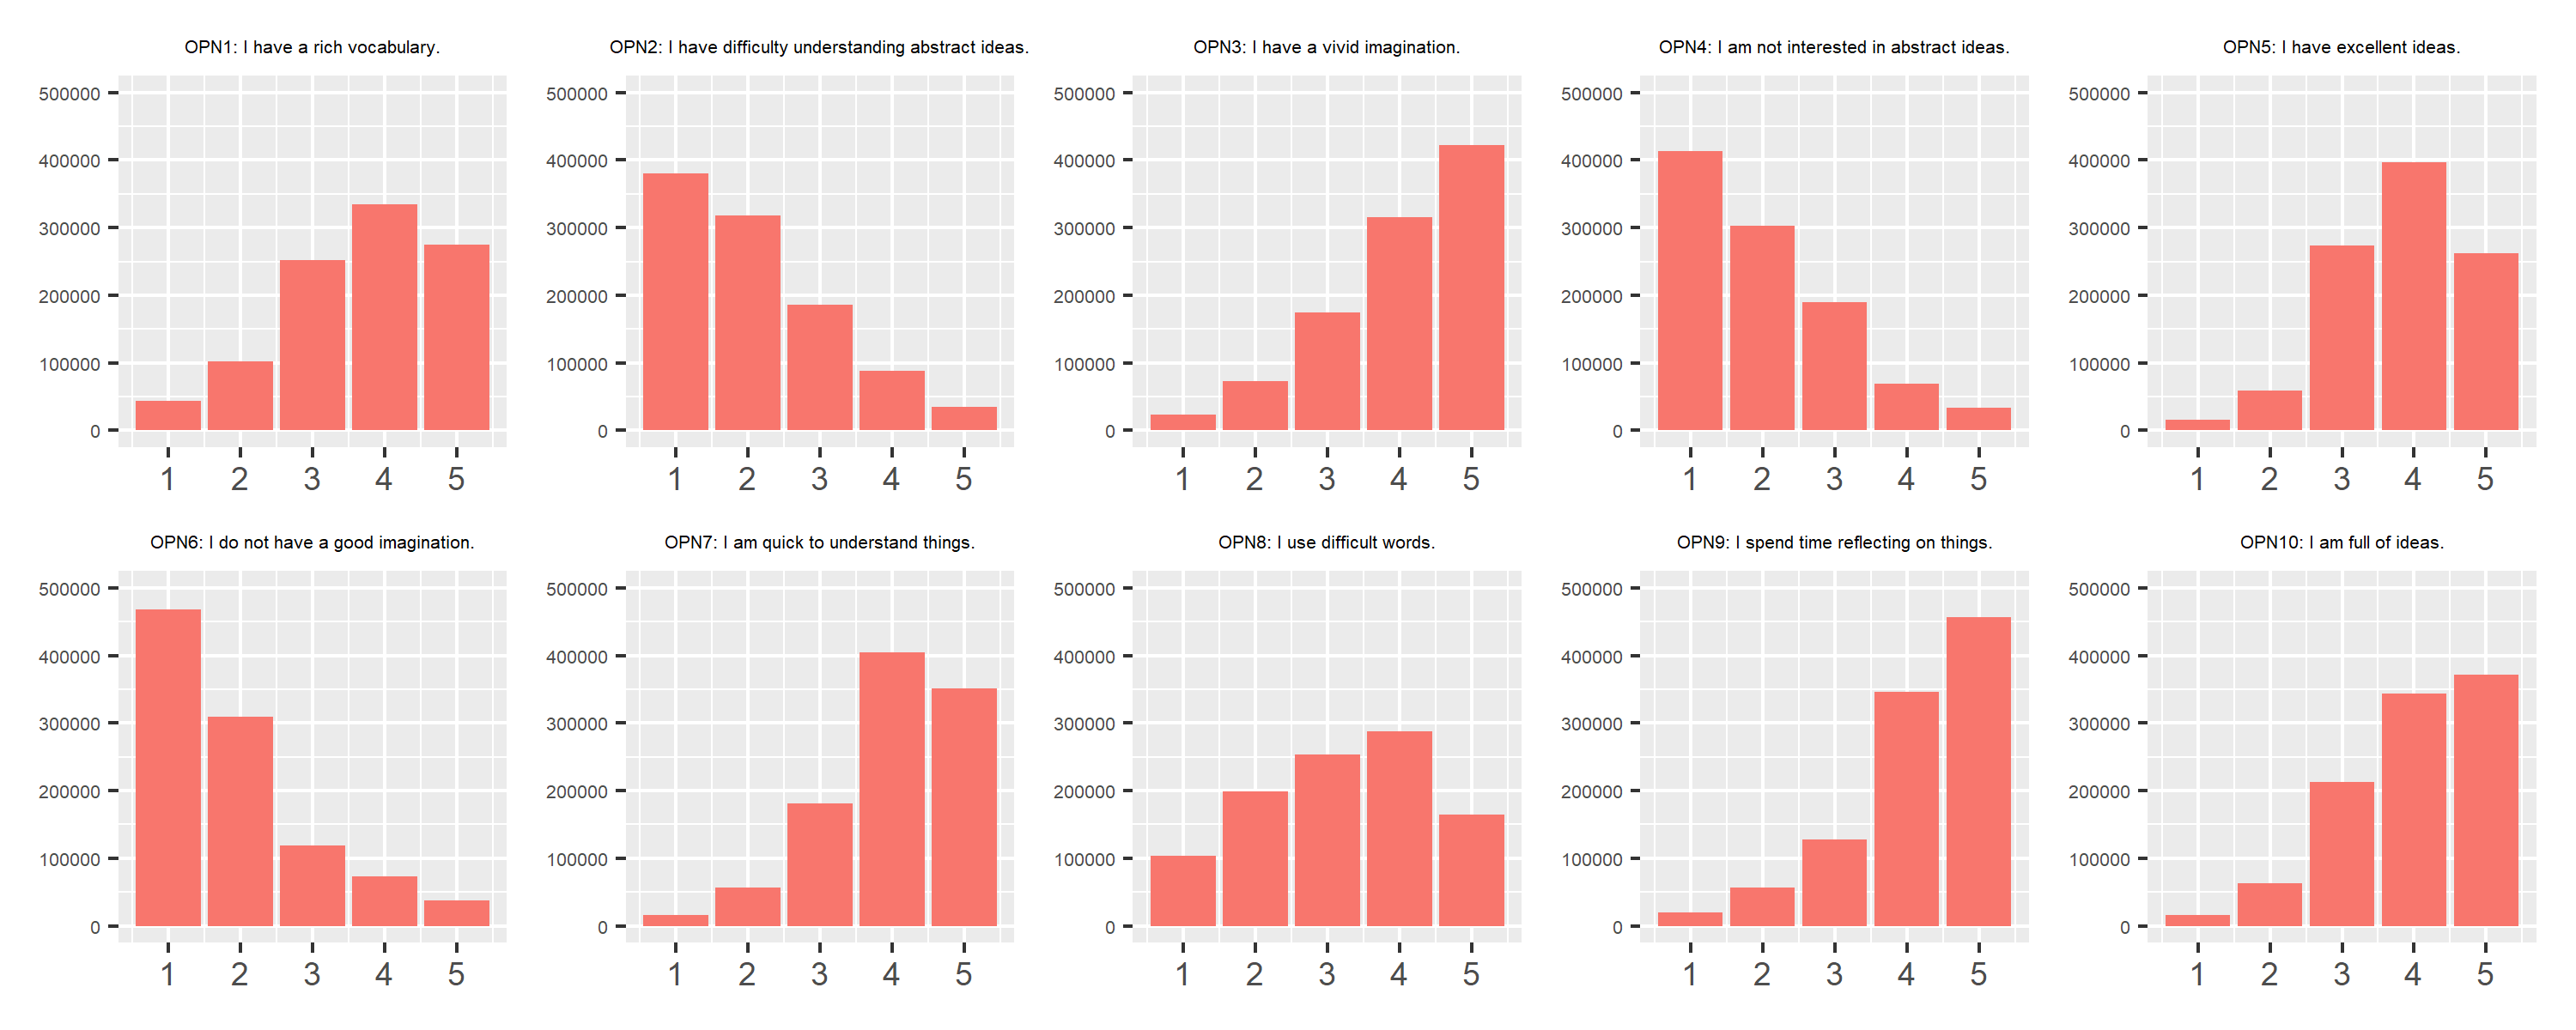
\includegraphics[scale=0.478]{OPN.png}
  \caption{开放性维度的题目及人数分布}
\end{figure}
\begin{figure}[H]
  \centering
  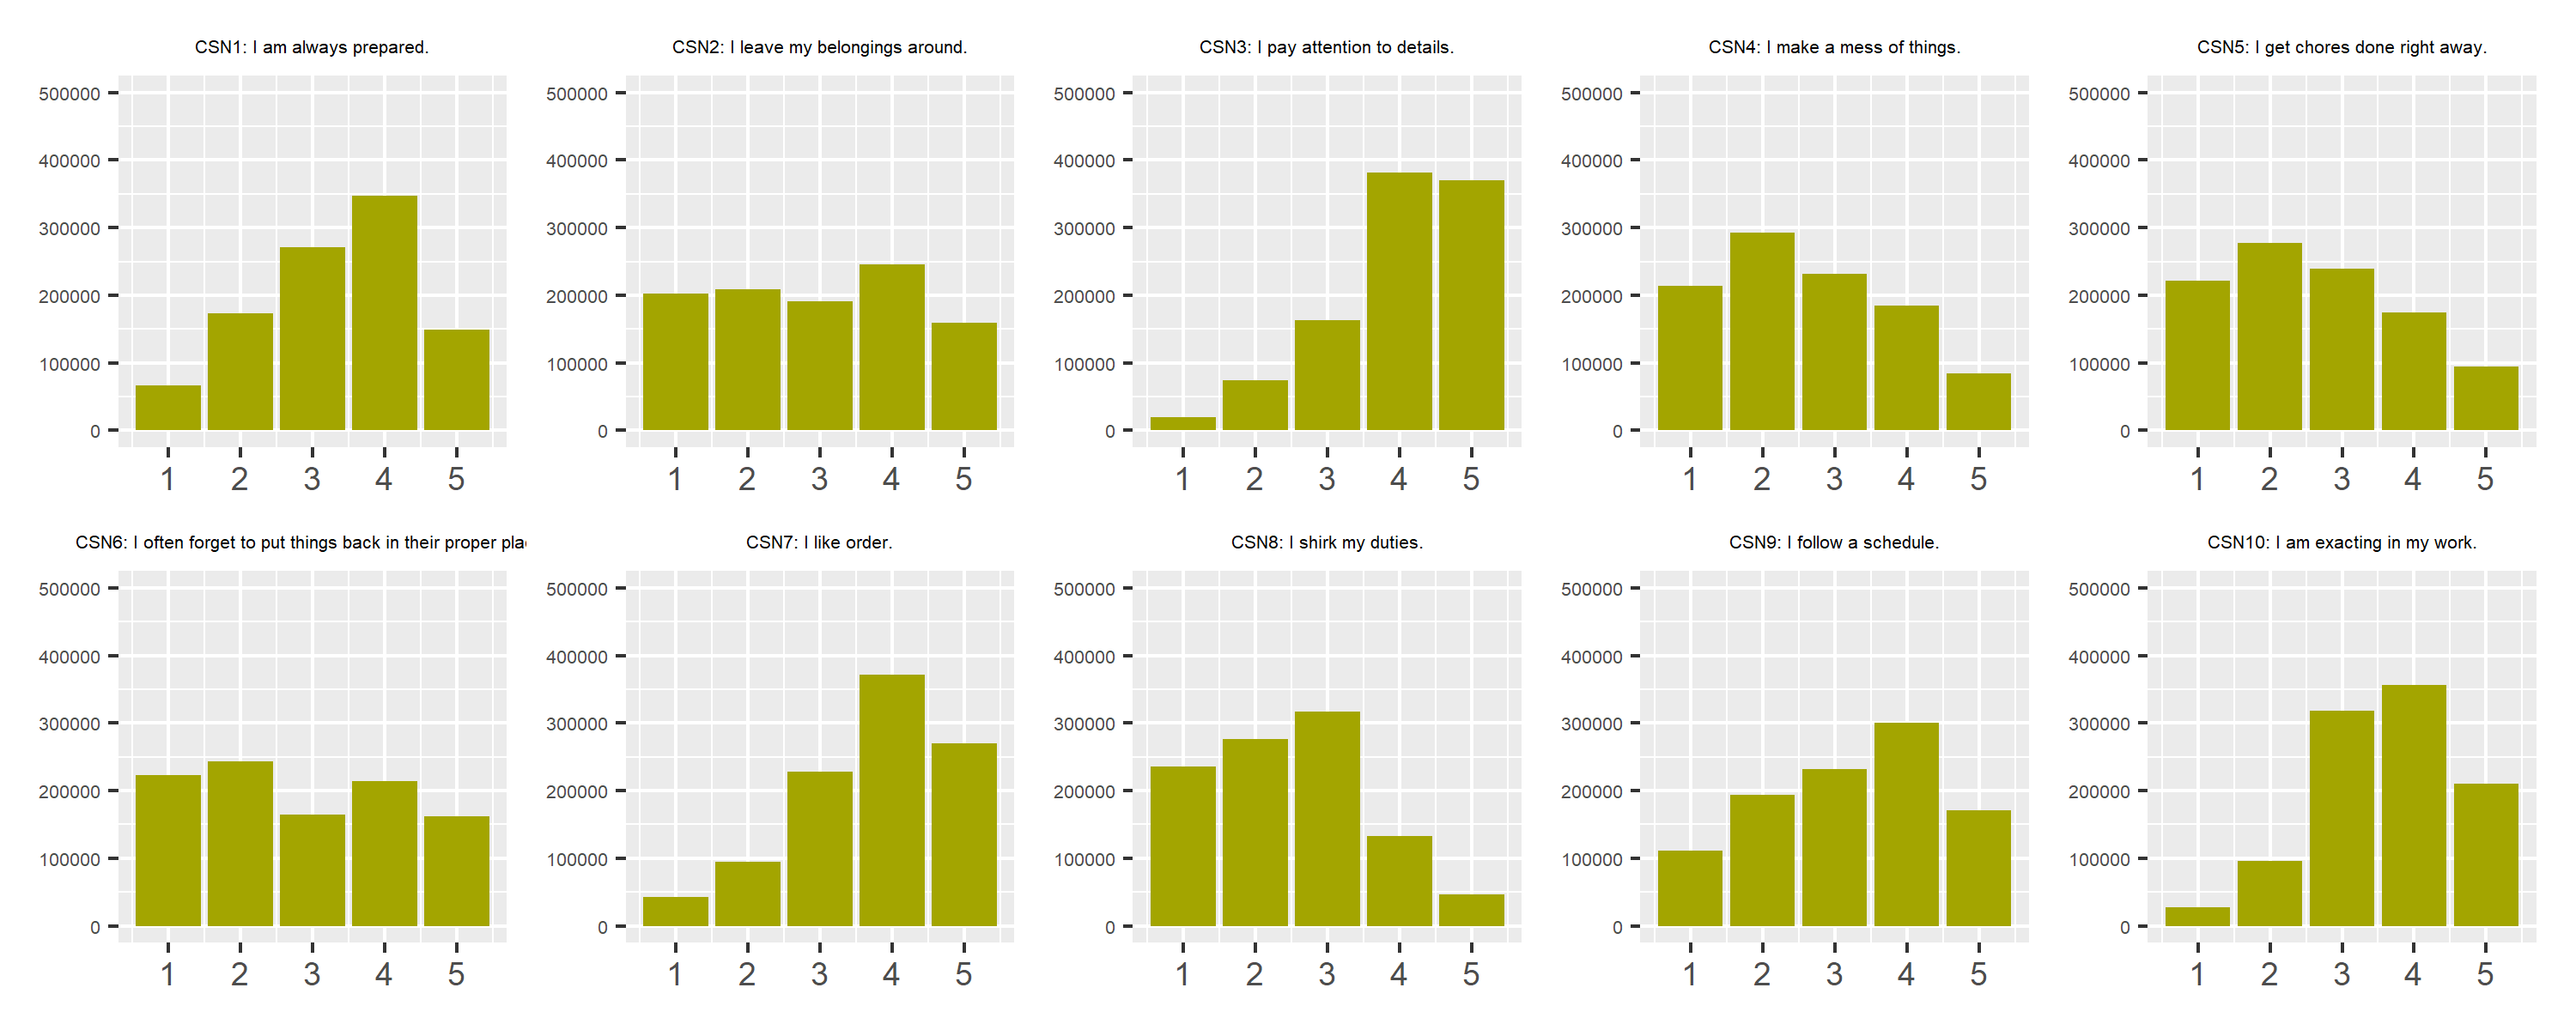
\includegraphics[scale=0.478]{CSN.png}
  \caption{尽责性维度的题目及人数分布}
\end{figure}
\begin{figure}[H]
  \centering
  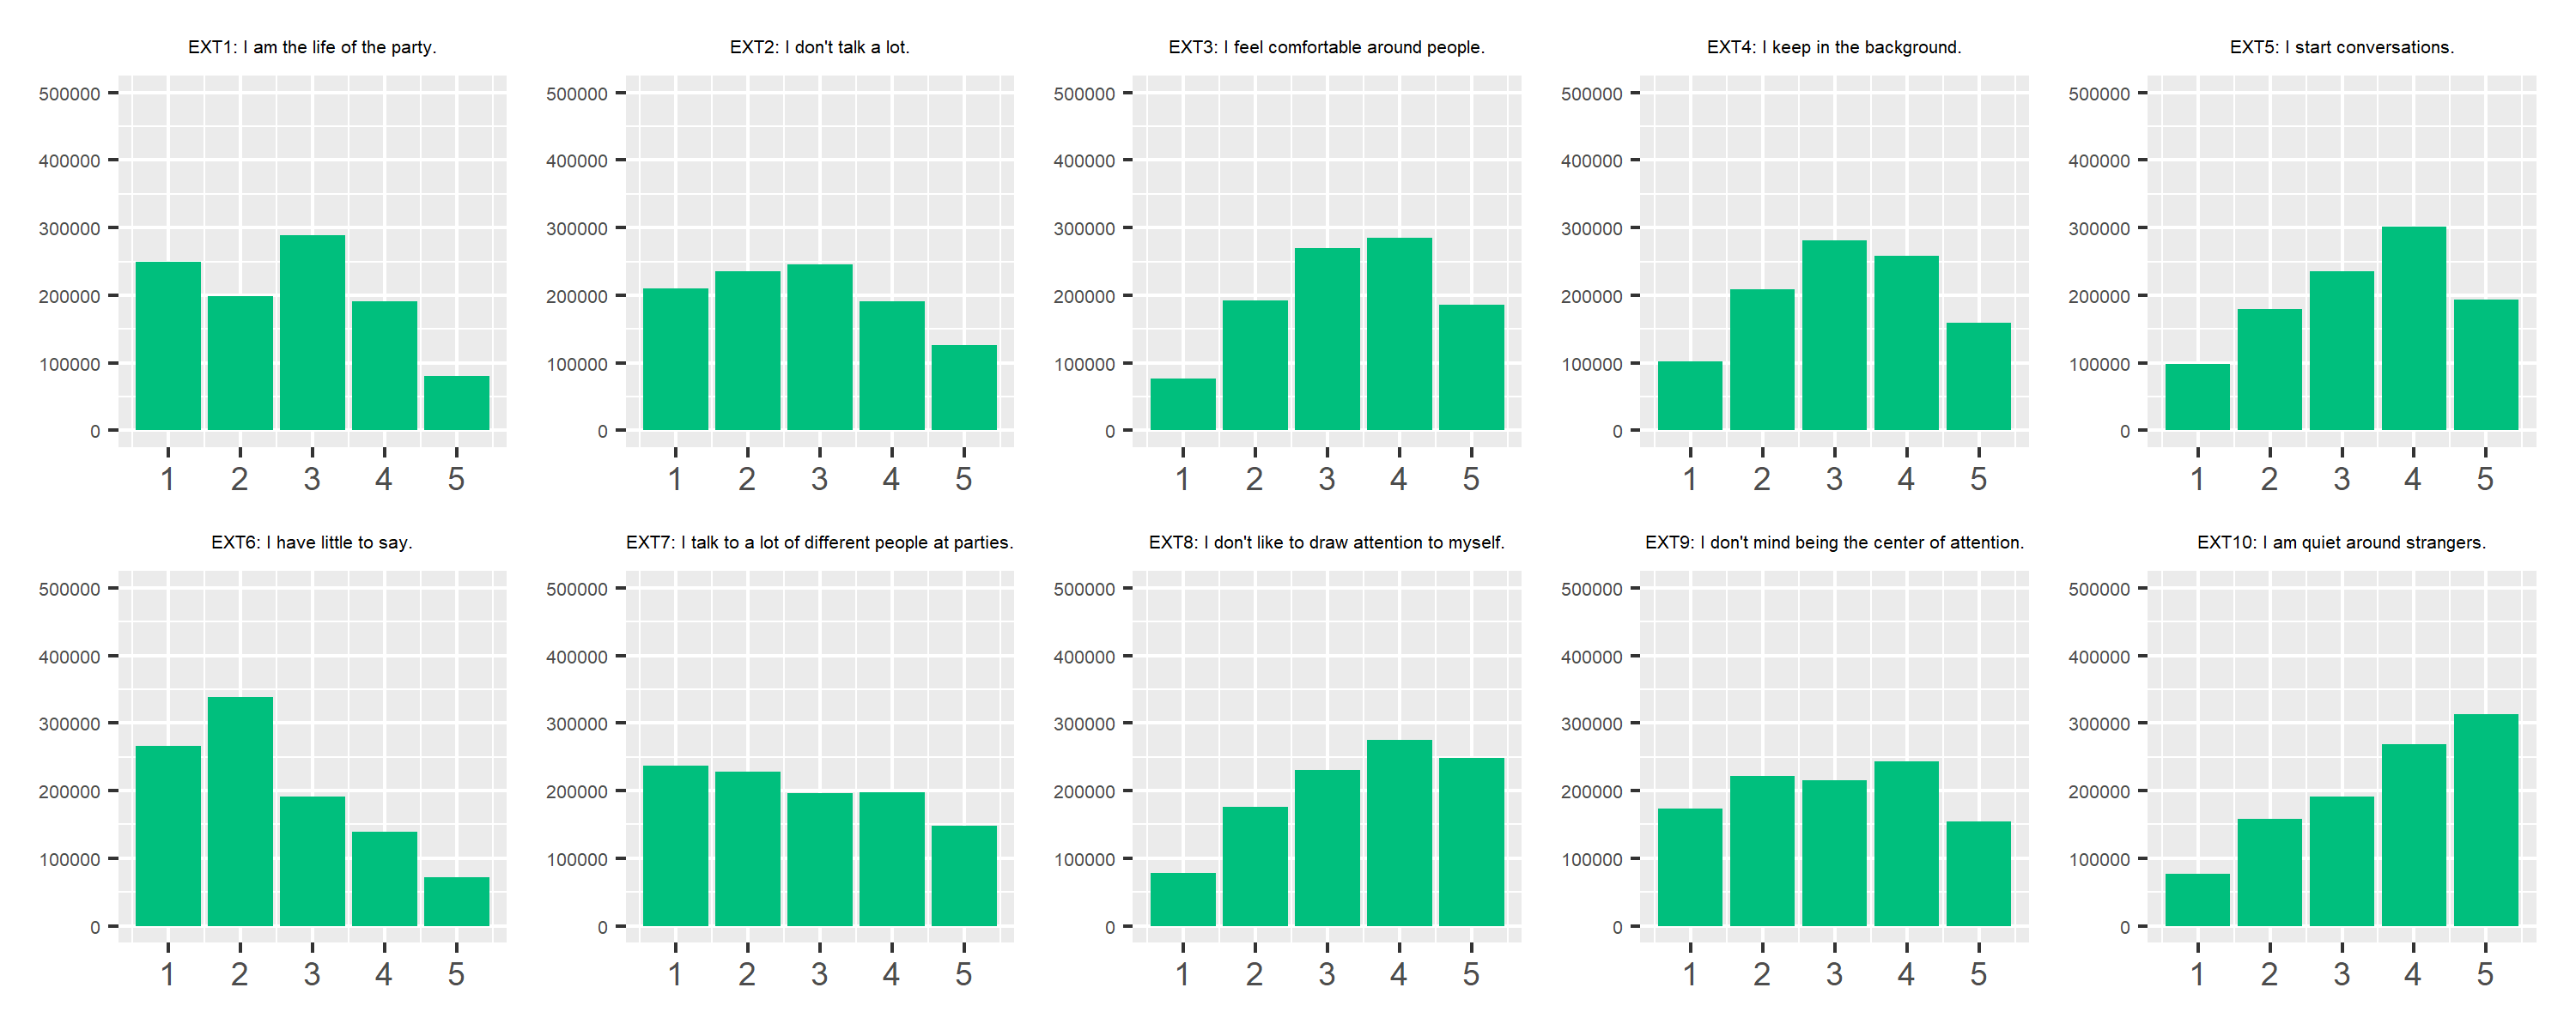
\includegraphics[scale=0.478]{EXT.png}
  \caption{外倾性维度的题目及人数分布}
\end{figure}
\begin{figure}[H]
  \centering
  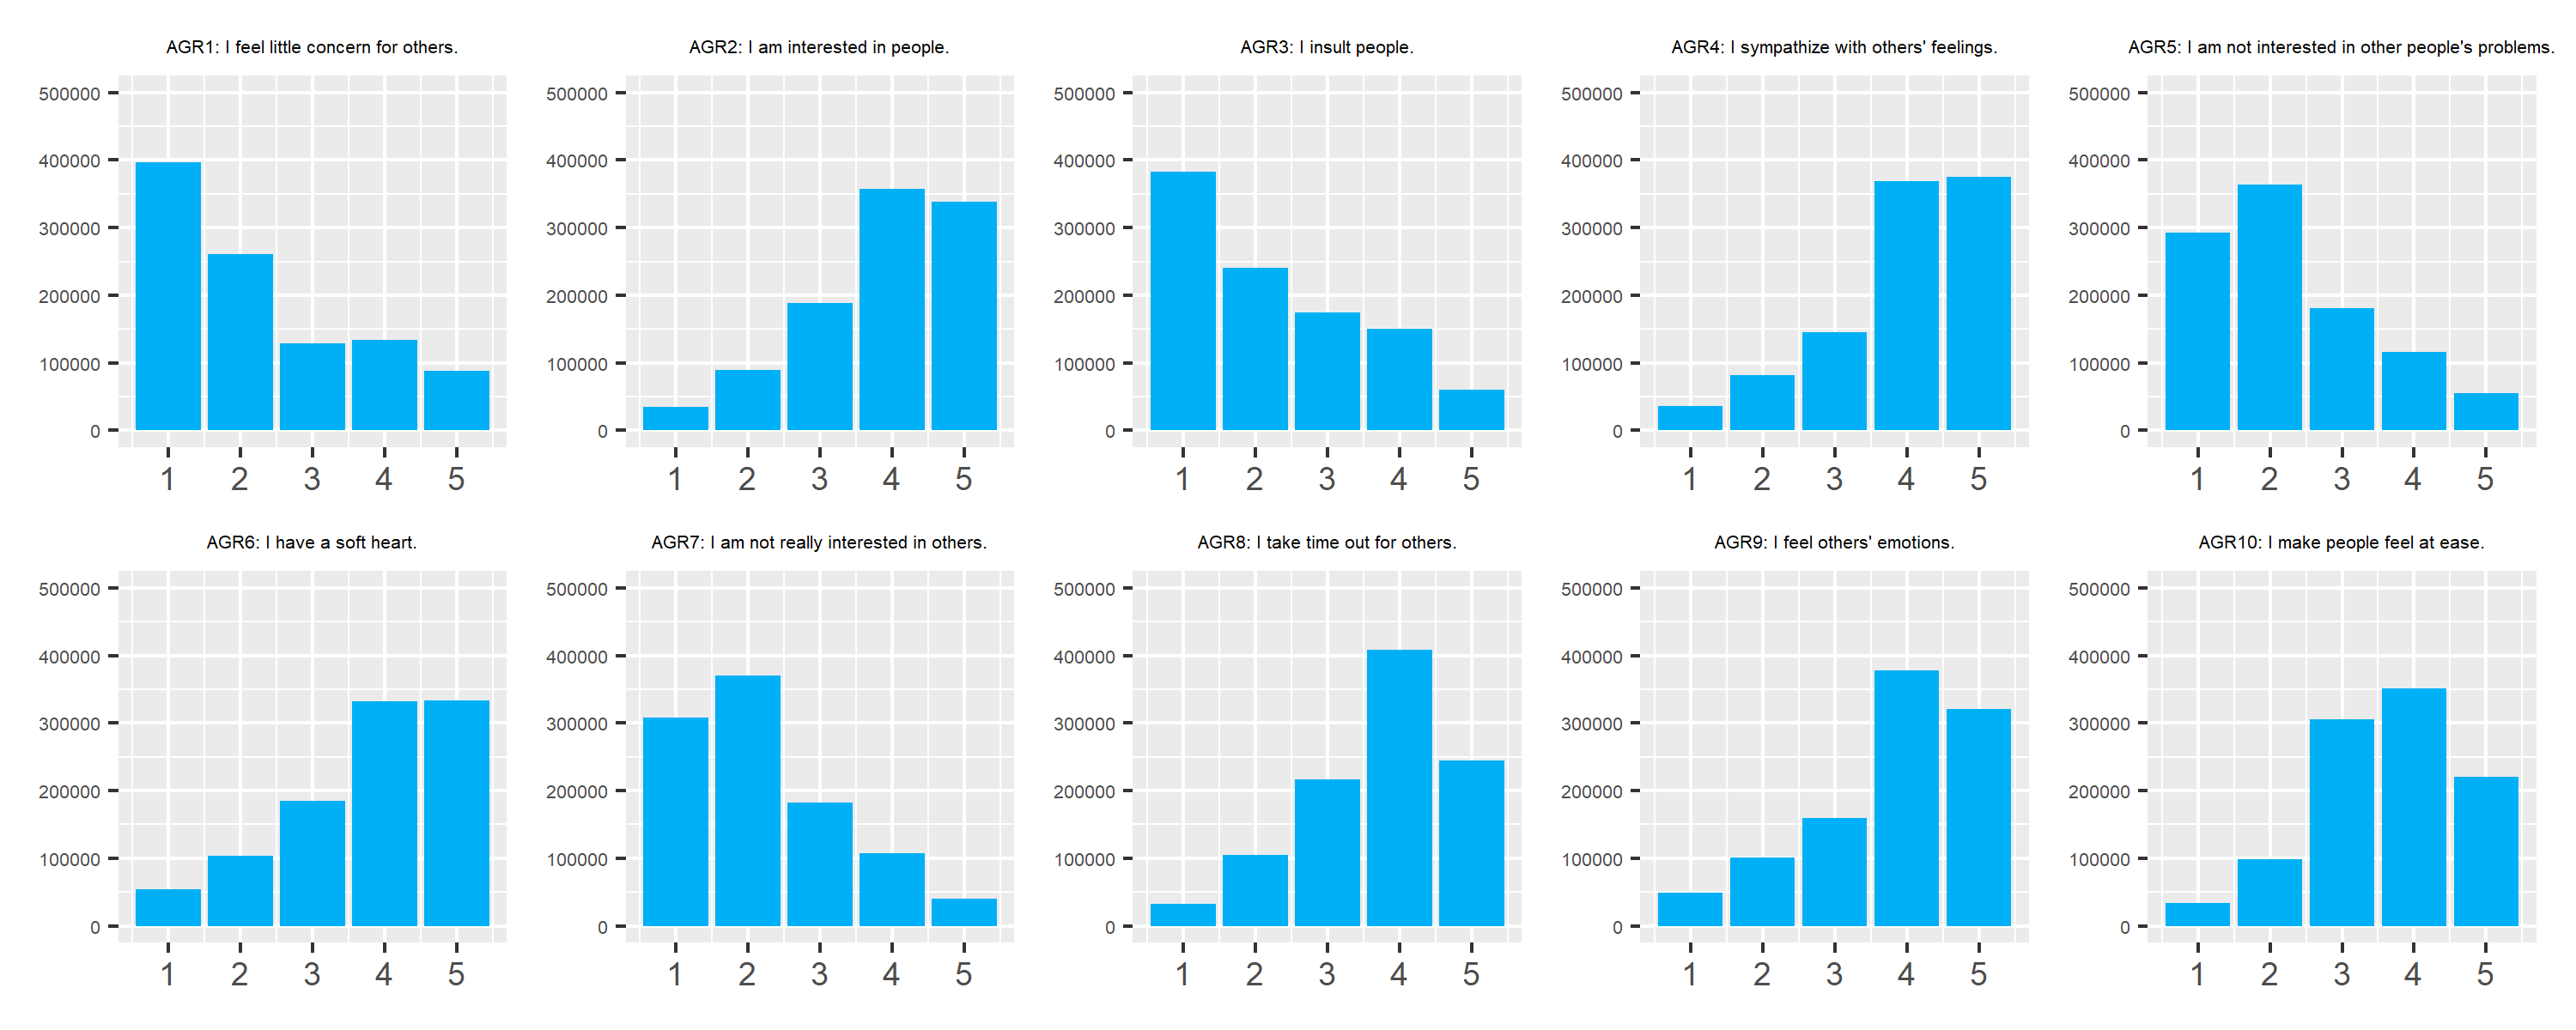
\includegraphics[scale=0.478]{AGR.png}
  \caption{宜人性维度的题目及人数分布}
\end{figure}
\begin{figure}[H]
  \centering
  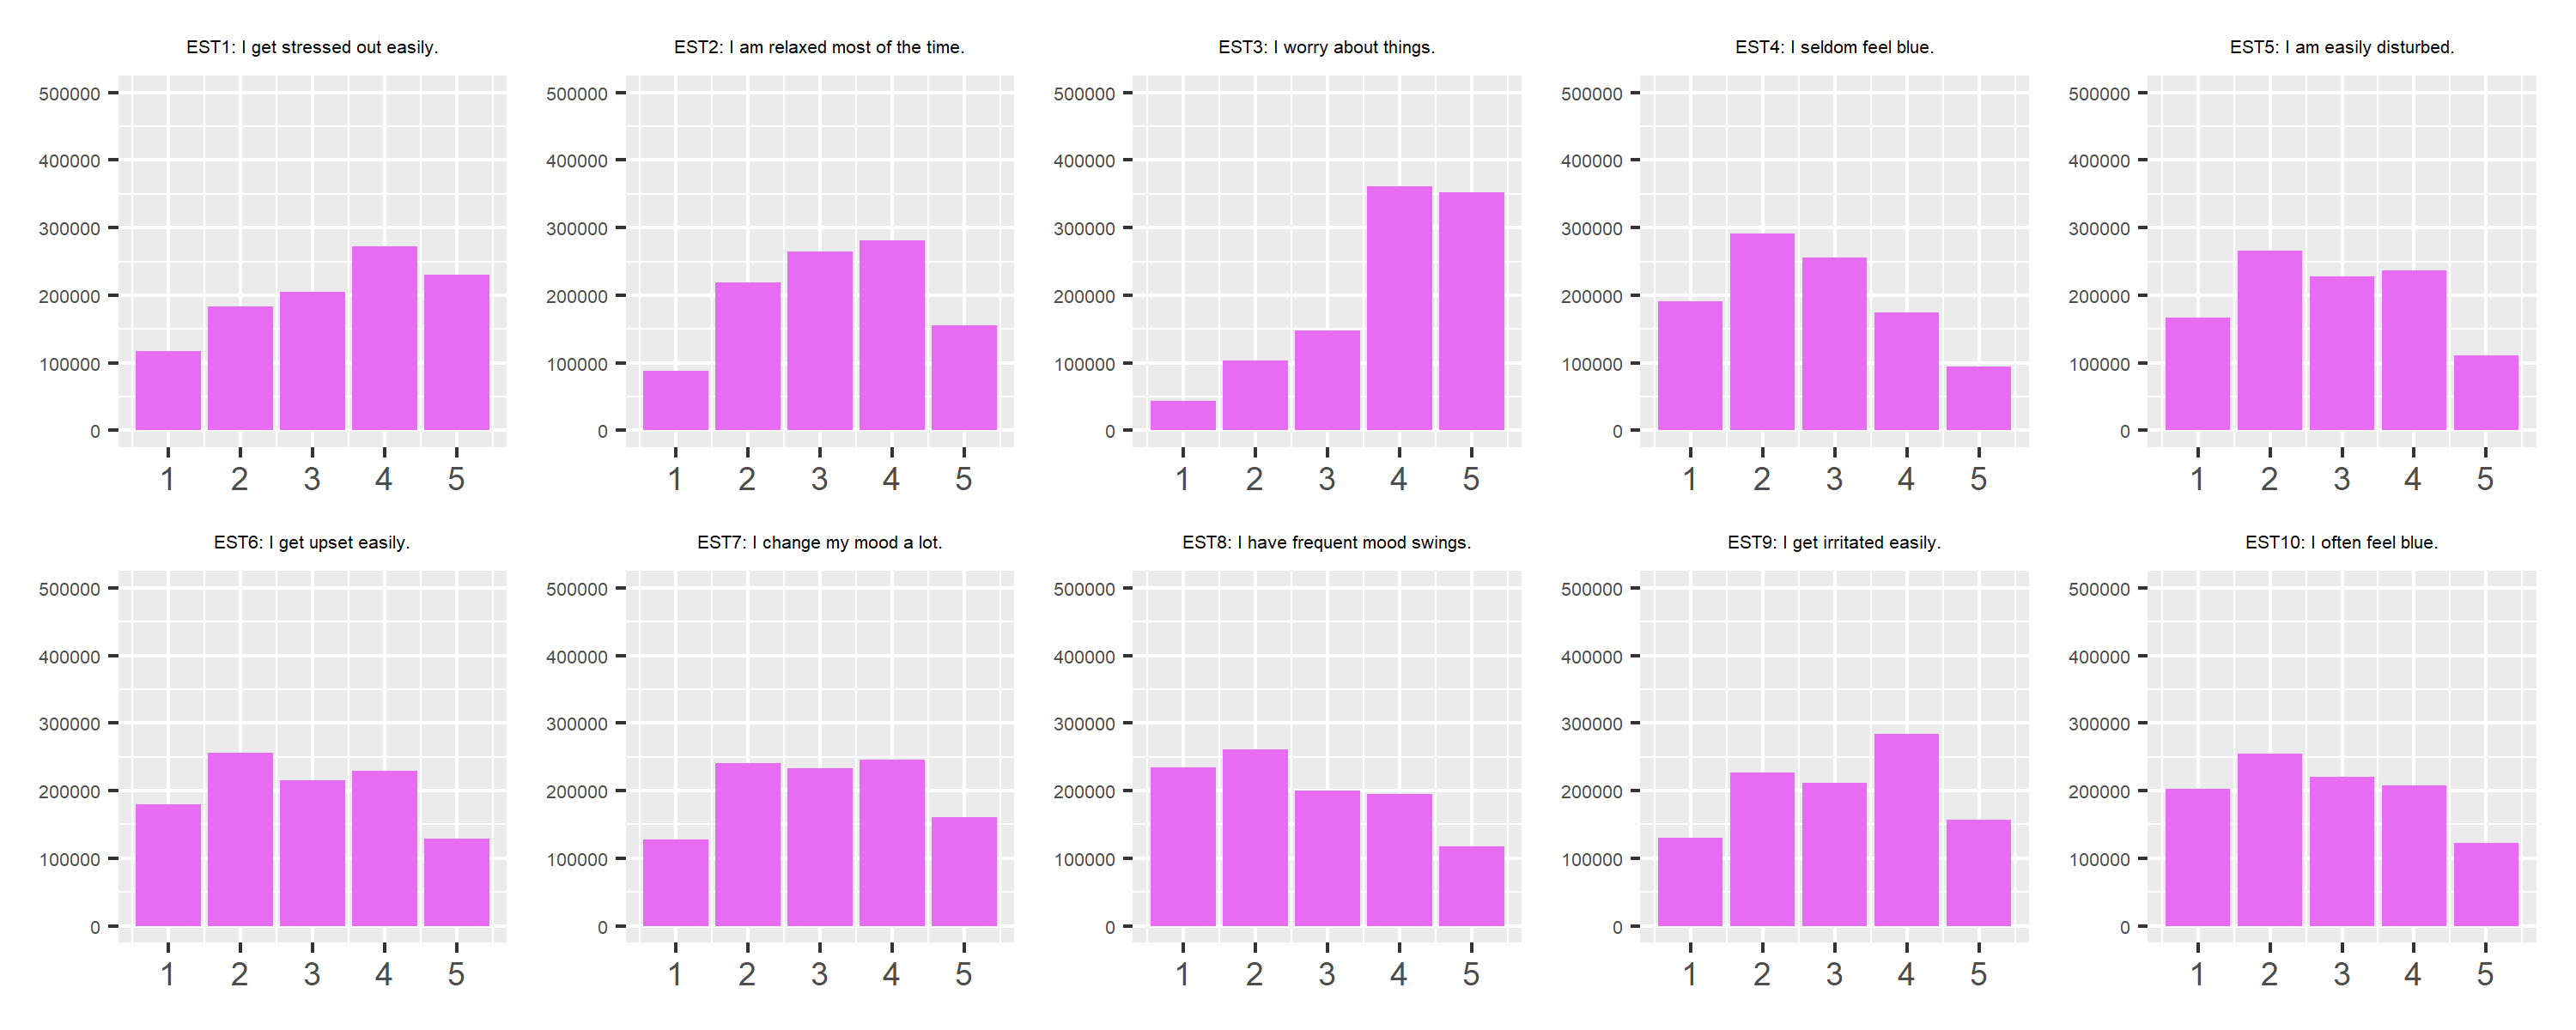
\includegraphics[scale=0.478]{EST.png}
  \caption{情绪性维度的题目及人数分布}
\end{figure}
可以看出,分布图像大致可分为5种形状:
\begin{itemize}
  \item 单调:按分数1$\sim$5呈单调递增或单调递减,顶部陡峭。
  \item 薄尾:峰值出现在分数2$\sim$4处,并向两侧快速递减,顶部较陡峭。
  \item 厚尾:峰值出现在分数2$\sim$4处,并向两侧缓慢递减,顶部较平坦。
  \item 平顶:分数在1$\sim$5中大约平均分布。
  \item 双峰:在分数1$\sim$2和4$\sim$5中各有一个峰值。
\end{itemize}\par
整理出所有题目以及分布类型的对照表如下:
\begin{longtable}{c|c|c}
  \hline
  \textbf{变量名} & \textbf{题目}                                              & \textbf{分布类型} \\\hline
  OPN1         & I have a rich vocabulary.                                & 薄尾            \\\hline
  OPN2         & I have difficulty understanding abstract ideas.          & 单调            \\\hline
  OPN3         & I have a vivid imagination.                              & 单调            \\\hline
  OPN4         & I am not interested in abstract ideas.                   & 单调            \\\hline
  OPN5         & I have excellent ideas.                                  & 薄尾            \\\hline
  OPN6         & I do not have a good imagination.                        & 单调            \\\hline
  OPN7         & I am quick to understand things.                         & 薄尾            \\\hline
  OPN8         & I use difficult words.                                   & 厚尾            \\\hline
  OPN9         & I spend time reflecting on things.                       & 单调            \\\hline
  OPN10        & I am full of ideas.                                      & 单调            \\\hline
  CSN1         & I am always prepared.                                    & 厚尾            \\\hline
  CSN2         & I leave my belongings around.                            & 平顶            \\\hline
  CSN3         & I pay attention to details.                              & 薄尾            \\\hline
  CSN4         & I make a mess of things.                                 & 厚尾            \\\hline
  CSN5         & I get chores done right away.                            & 厚尾            \\\hline
  CSN6         & I often forget to put things back in their proper place. & 双峰            \\\hline
  CSN7         & I like order.                                            & 薄尾            \\\hline
  CSN8         & I shirk my duties.                                       & 厚尾            \\\hline
  CSN9         & I follow a schedule.                                     & 厚尾            \\\hline
  CSN10        & I am exacting in my work.                                & 薄尾            \\\hline
  EXT1         & I am the life of the party.                              & 双峰            \\\hline
  EXT2         & I don't talk a lot.                                      & 厚尾            \\\hline
  EXT3         & I feel comfortable around people.                        & 厚尾            \\\hline
  EXT4         & I keep in the background.                                & 厚尾            \\\hline
  EXT5         & I start conversations.                                   & 厚尾            \\\hline
  EXT6         & I have little to say.                                    & 薄尾            \\\hline
  EXT7         & I talk to a lot of different people at parties.          & 平顶            \\\hline
  EXT8         & I don't like to draw attention to myself.                & 厚尾            \\\hline
  EXT9         & I don't mind being the center of attention.              & 平顶            \\\hline
  EXT10        & I am quiet around strangers.                             & 单调            \\\hline
  AGR1         & I feel little concern for others.                        & 单调            \\\hline
  AGR2         & I am interested in people.                               & 薄尾            \\\hline
  AGR3         & I insult people.                                         & 单调            \\\hline
  AGR4         & I sympathize with others' feelings.                      & 单调            \\\hline
  AGR5         & I am not interested in other people's problems.          & 薄尾            \\\hline
  AGR6         & I have a soft heart.                                     & 单调            \\\hline
  AGR7         & I am not really interested in others.                    & 薄尾            \\\hline
  AGR8         & I take time out for others.                              & 薄尾            \\\hline
  AGR9         & I feel others' emotions.                                 & 薄尾            \\\hline
  AGR10        & I make people feel at ease.                              & 薄尾            \\\hline
  EST1         & I get stressed out easily.                               & 厚尾            \\\hline
  EST2         & I am relaxed most of the time.                           & 厚尾            \\\hline
  EST3         & I worry about things.                                    & 薄尾            \\\hline
  EST4         & I seldom feel blue.                                      & 厚尾            \\\hline
  EST5         & I am easily disturbed.                                   & 双峰            \\\hline
  EST6         & I get upset easily.                                      & 双峰            \\\hline
  EST7         & I change my mood a lot.                                  & 平顶            \\\hline
  EST8         & I have frequent mood swings.                             & 厚尾            \\\hline
  EST9         & I get irritated easily.                                  & 双峰            \\\hline
  EST10        & I often feel blue.                                       & 厚尾            \\\hline
  \caption{题目及人数分布类型}
  \label{type}
\end{longtable}\par
其中,仅厚尾、平顶和双峰形状可近似看成分数集中于3附近,单调和薄尾形状的人数分布均偏向一端,
二者的比例恰好为$1:1$。这说明相当一部分题目具有导向性,参加测验的人会更倾向选择符合或不符合的一端。
此外,每个维度中问题的分布类型也有各自的特点:
\begin{itemize}
  \item 开放性维度题目的分布类型为单调和薄尾,人数分布差异很大。
  \item 尽责性维度题目的分布类型多为厚尾和薄尾,人数分布比较均匀。
  \item 外倾性维度题目的分布类型多为厚尾和平顶,人数分布很均匀。
  \item 宜人性维度题目的分布类型为薄尾和单调,人数分布差异很大。
  \item 情绪性维度题目的分布类型多为厚尾和双峰,人数分布很均匀。
\end{itemize}
因此,对于开放性和宜人性,大多数人可能有同样的高分或低分倾向,区分度不高;
而尽责性、外倾性和情绪性由于各分数分布较均匀,可能才是更明显地体现出人格特质差异的重要维度。
% 一个比较有意思的情况是,不少相近叙述或反向叙述的题目具有不同的分布类型,
% 比如EXT2和EXT6(厚尾和薄尾)、AGR4和AGR9(单调和薄尾)。
% 这说明在改变题目叙述方式后,有相当一部分人的倾向选择也发生了变化。
% 这种变化差异也许就是人们具有人格特质差异的表现,也从侧面体现了题目设置的巧妙之处。
\section{维度和题目的相关性分析}
% 对于一对相近或反向叙述的题目,理应具有比较高的正相关性或负相关性,
% 但是人数分布的图像显示并不完全是这样,即图像不属于同一种形状。\par
\begin{figure}[H]
  \centering
  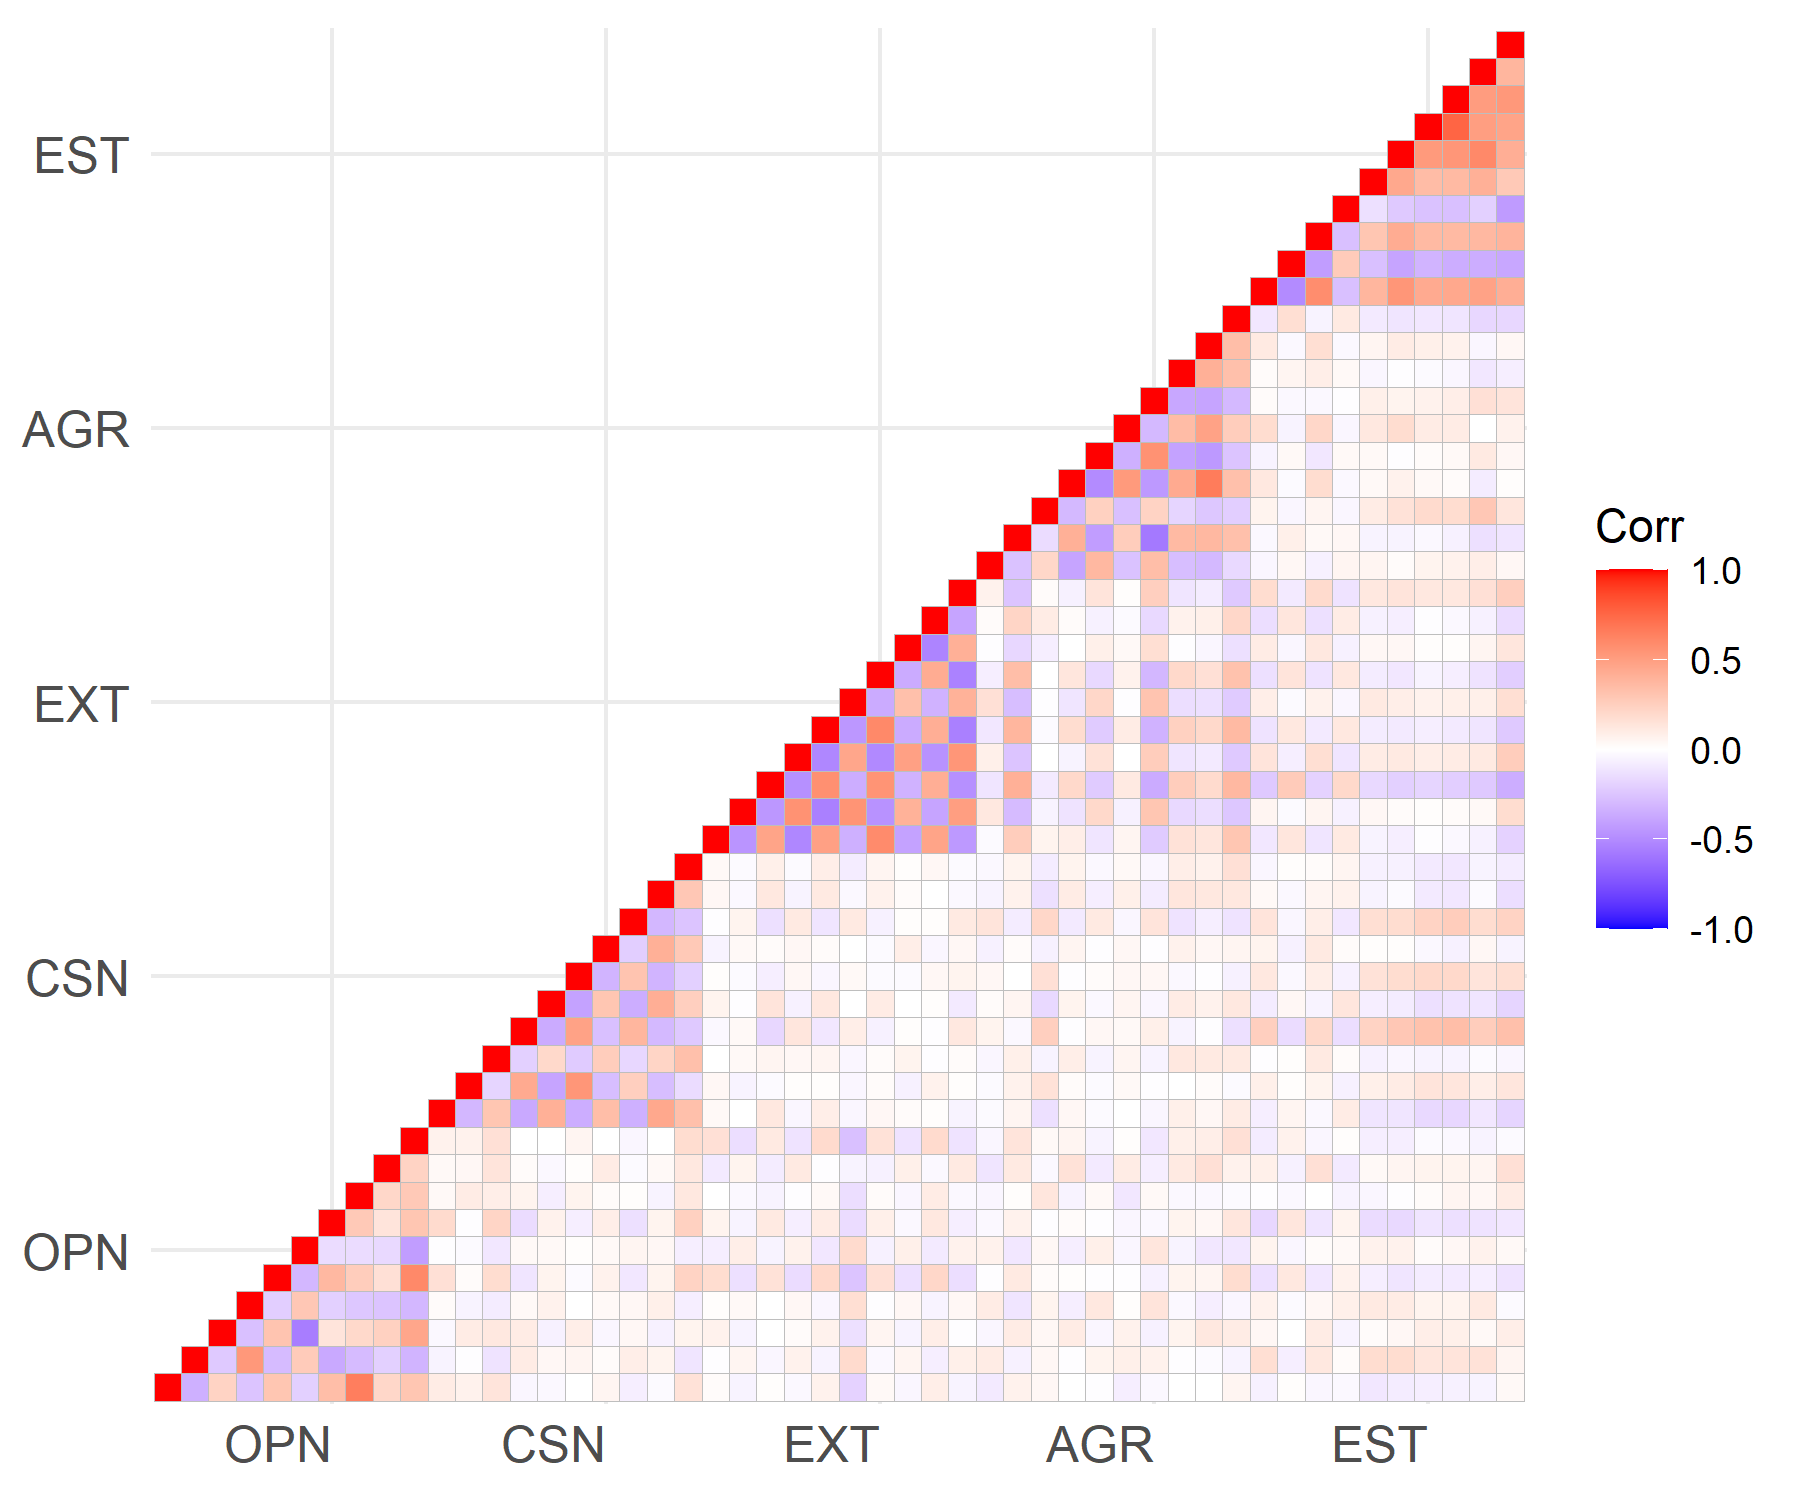
\includegraphics[scale=0.7]{Corrplot_Item.png}
  \caption{题目间的相关系数}
\end{figure}
通过计算关于题目分数之间的相关系数,画出相关系数矩阵图。
图像显示,同一维度的题目之间具有较明显的相关性,而不同维度的题目之间则相关性较低。
这样的特点符合大五人格测验使用10个题目的分数计算一个维度的人格特质倾向的模式,
也证明了同一维度中确实存在相关性比较高的相似题目或反向题目。\par
% 对于前面文字描述上关联性较强的题目,其相关系数分别为:
% \begin{longtable}{c|c|c|c|c}
%   \hline
%   题目&CSN4-CSN6&EXT2-EXT6&AGR4-AGR9&EST6-EST10\\\hline
%   相关系数&0.4810&0.5469&0.6579&0.4241\\\hline
% \end{longtable}
同时发现,在外倾性(EXT)和宜人性(AGR)、外倾性(EXT)和情绪性(EST)、
尽责性(CSN)和情绪性(EST)的部分题目之间也存在一定的相关性,
其中部分题目间的相关系数达到$0.4$以上。\par
\begin{figure}[H]
  \centering
  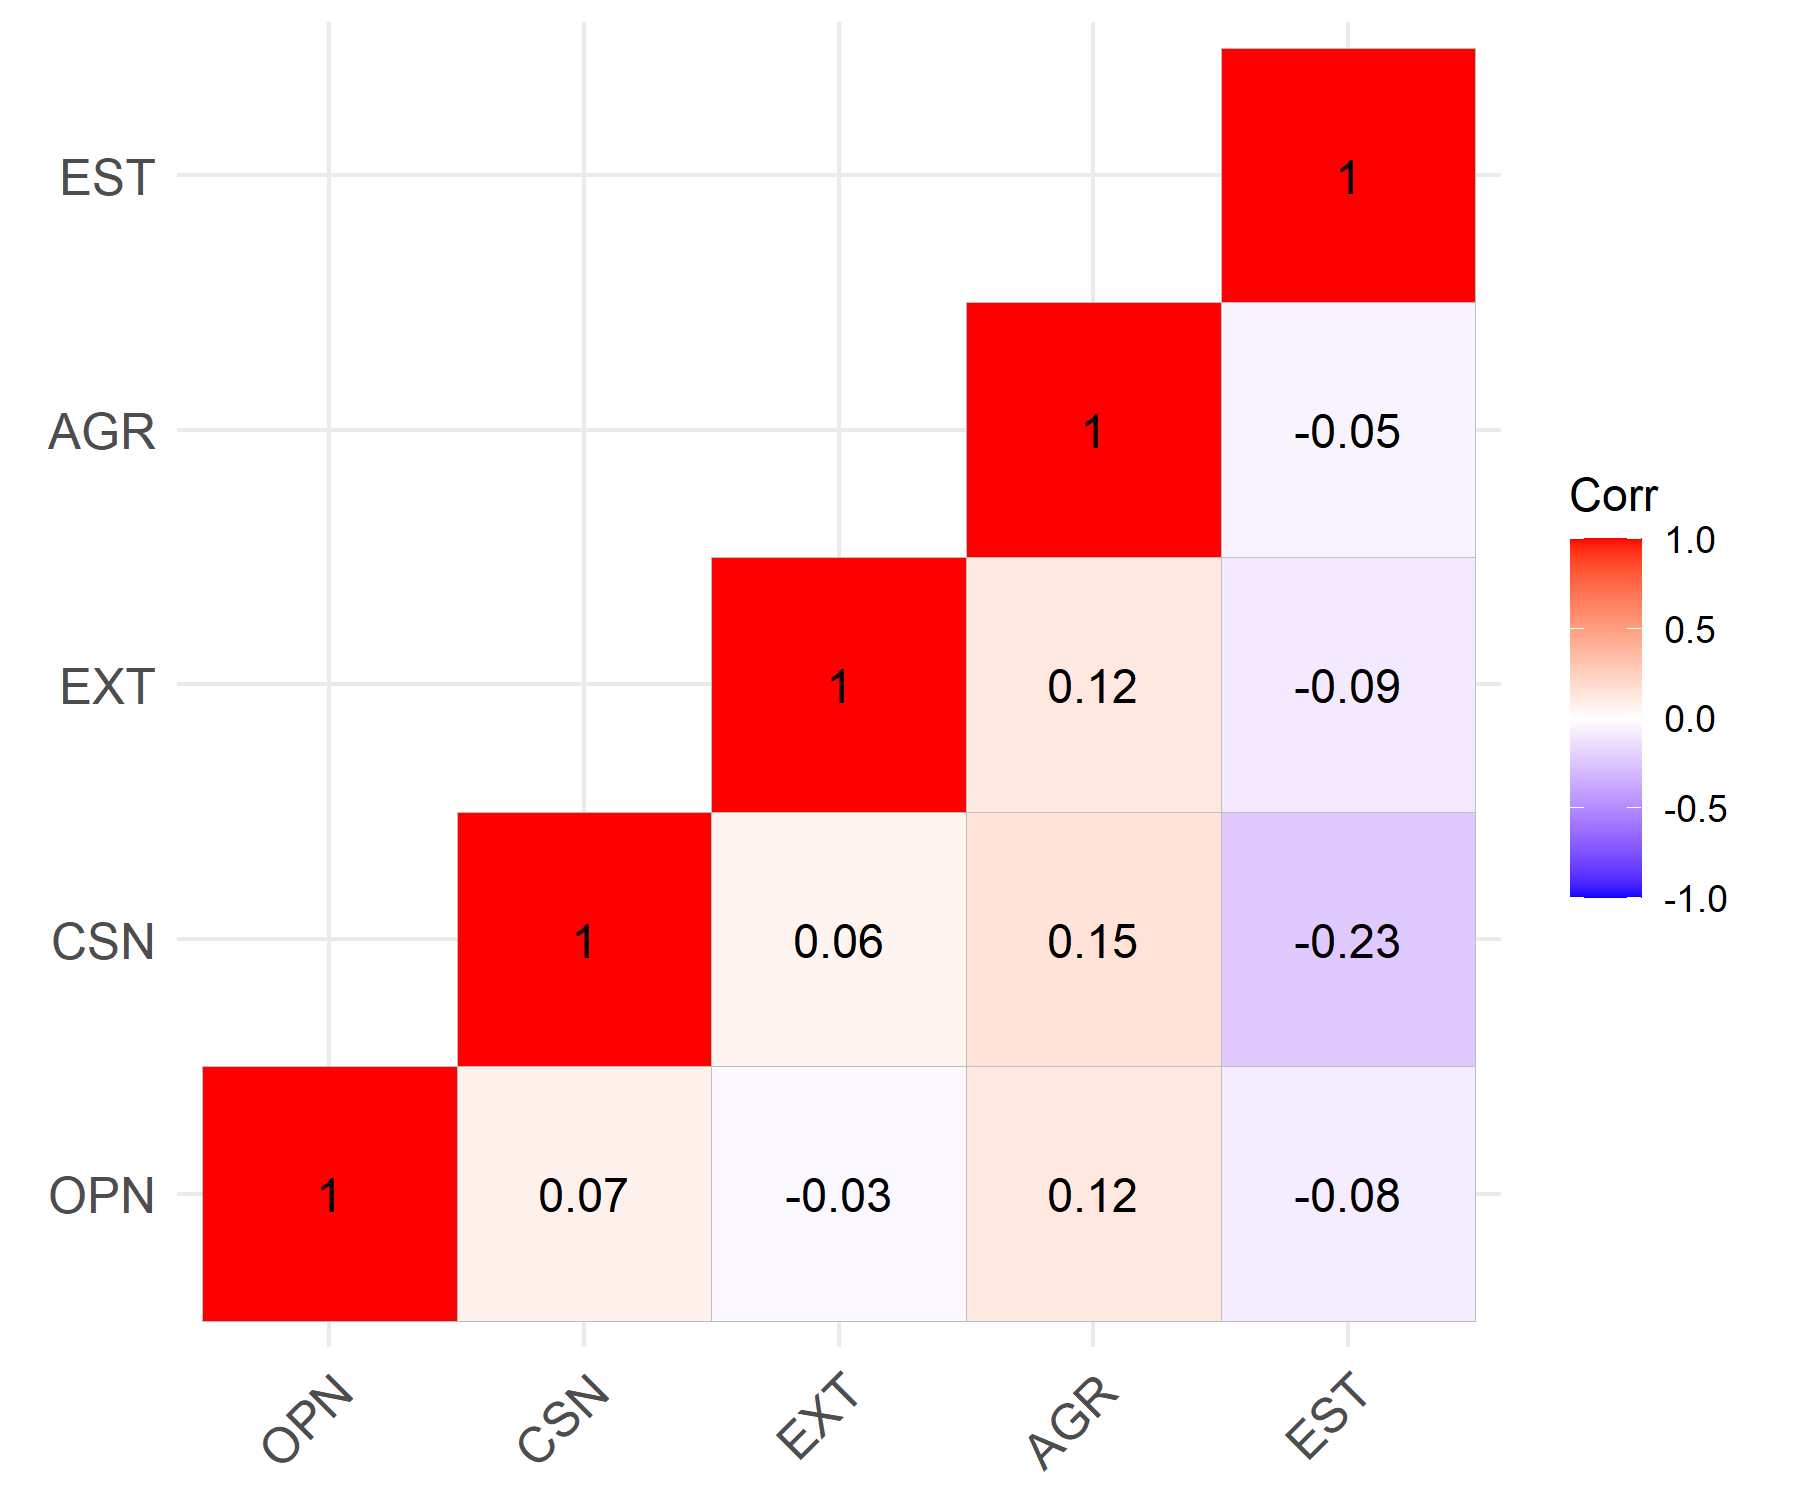
\includegraphics[scale=0.7]{Corrplot_Dimension.png}
  \caption{维度间的相关系数}
\end{figure}
将反向记分的题目处理后,计算每个维度下10道题目总分的相关系数,画出相关系数矩阵图。
图像显示,不同维度总分的相关系数均在一个很低的水平。
其中,尽责性(CSN)和情绪性(EST)是唯一相关系数超过0.2的负相关,
一种合理的解释是一个责任感强的人可能会更冷静,更不容易有情绪化反应。\par
综上所述,虽然跨维度的题目间存在一些低度相关的情况,但维度总分之间仅存在微弱相关,
使用维度总分作为人格特质倾向性的量化分数是客观、有效的。
\section{参加者的国家分布}
除去国籍未知的情况,数据中的参加测验的人共来自222个国家,
其中参加人数超过$10,000$人的国家有12个。
\begin{figure}[H]
  \centering
  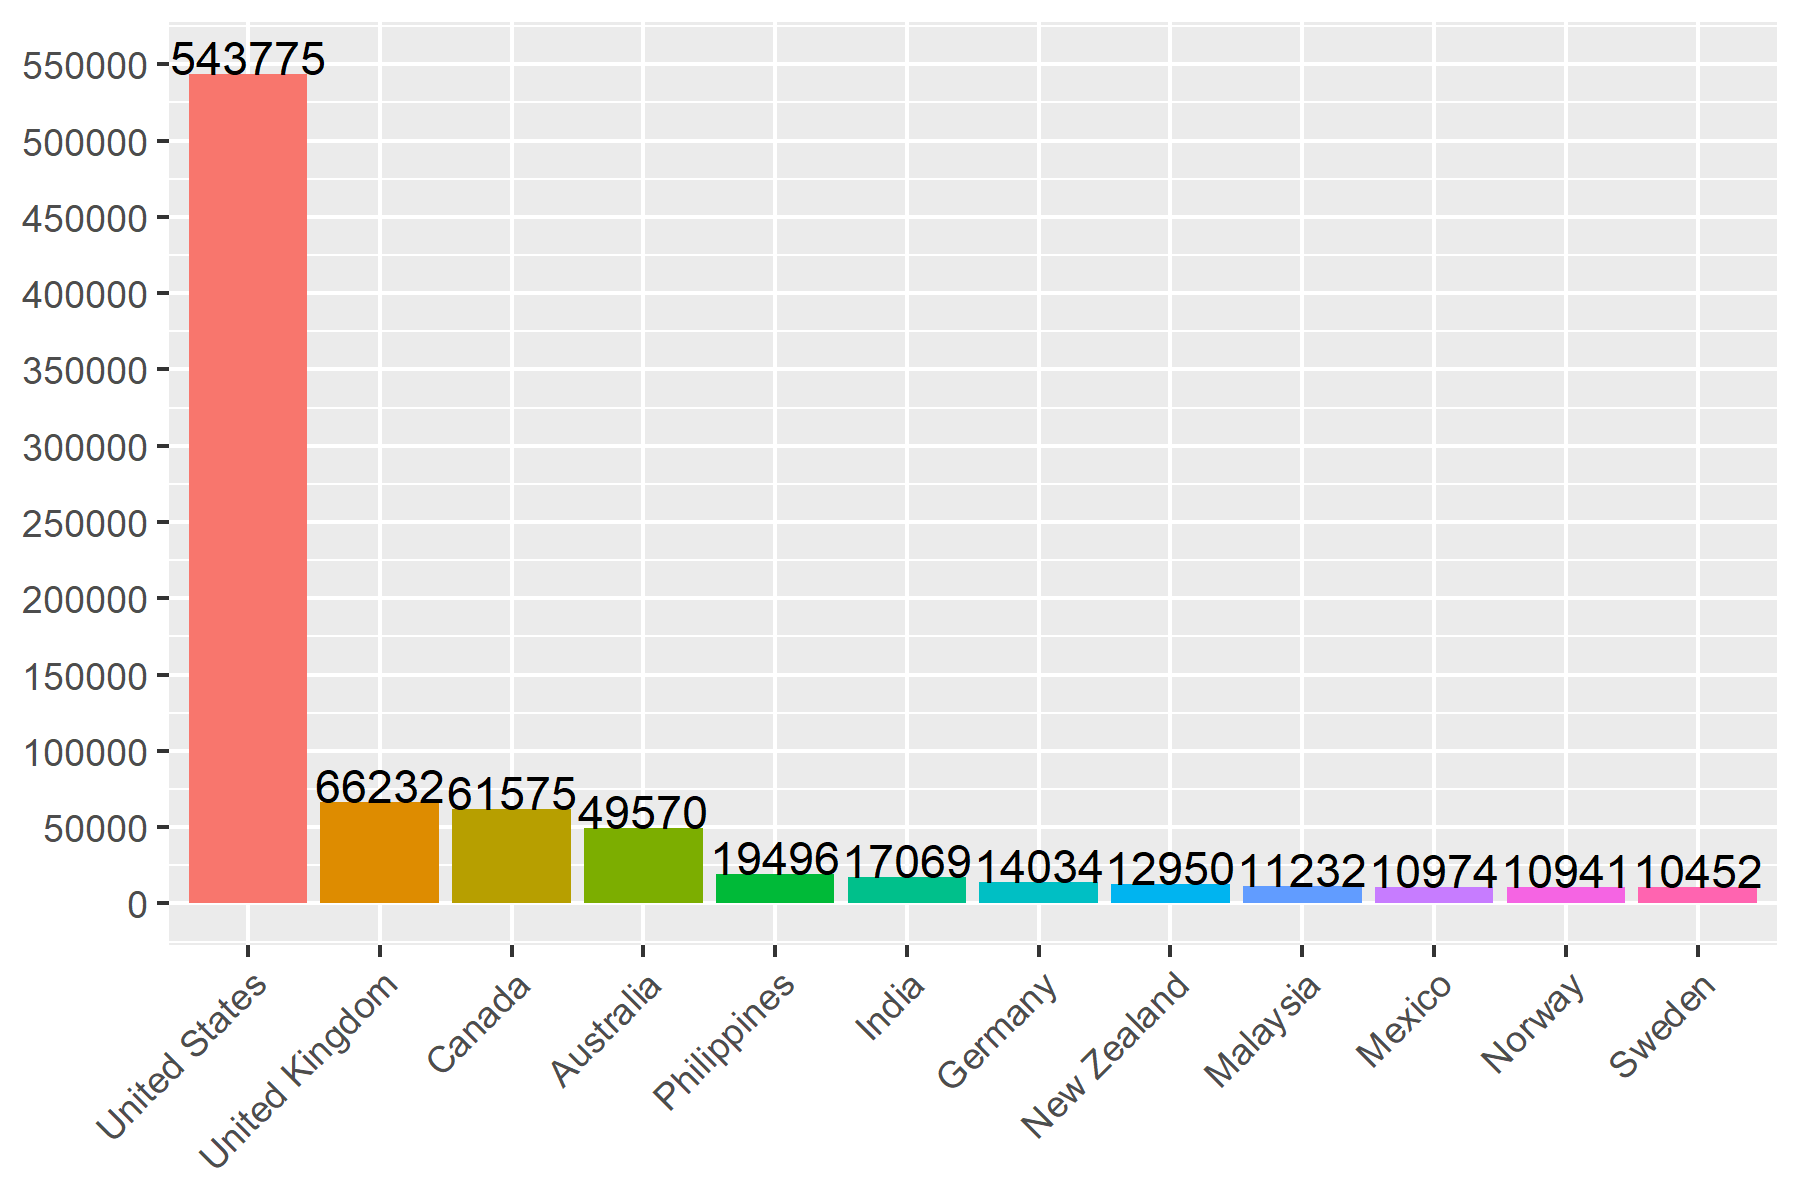
\includegraphics[scale=0.79]{Country.png}
  \caption{参加测验人数超过$10,000$的国家}
\end{figure}
全部样本中,来自美国的参加者占了一半以上,其余国家的人数均显著小于美国,
甚至绝大部分国家的参加者不足$10,000$人。
如果以平均倾向得分代表该国的人格特质倾向,那么该数据对于美国人的特质倾向将是比较好的研究材料,
研究其他参加者较少的国家时可能会因为样本量较少而出现偏差。
因此,在比较国家之间的人格特质差异时,将主要针对参加者人数较多的国家,人数较少的国家结果仅供参考。
\part{维度与分布类型的独立性检验}
% \setcounter{section}{0}
% \section{人数分布类型统计}
根据表\ref{type}可知,分布类型在各维度之间并不是随机出现的,每个维度都有各自的人数分布特点。
统计每个维度中的不同分布类型的个数,得到下表:
\begin{longtable}{c|c|c|c|c|c}
  \hline
  维度  & 单调 & 薄尾 & 厚尾 & 平顶 & 双峰 \\\hline
  OPN & 6  & 3  & 1  & 0  & 0  \\
  CSN & 0  & 3  & 5  & 1  & 1  \\
  EXT & 1  & 1  & 5  & 2  & 1  \\
  AGR & 4  & 6  & 0  & 0  & 0  \\
  EST & 0  & 1  & 5  & 1  & 3  \\\hline
  \caption{维度与分布类型列联表}
\end{longtable}
为了分析维度与分布类型是否有联系,对其进行卡方独立性检验。
由于表中部分单元格数值太小,直接计算出卡方统计量很可能不准确,
因此采用2000次蒙特卡罗模拟的结果进行卡方检验,检验结果如下:
\begin{longtable}{c|c}
  \hline
  X-squared & 36.341   \\\hline
  p-value   & 0.000995 \\\hline
  \caption{维度与分布类型的卡方独立性检验(基于2000次蒙特卡罗模拟)}
\end{longtable}
因为p值相当小,所以认为维度与人数分布类型不是相互独立的。
人们在不同维度的题目下有不同的倾向性选择,说明五个维度在构成完整的人格特质时的作用是不同的,
五个维度分别描述的是五个不同的方面,一个人在这五个方面上的不同表现组成了他的完整人格。
\part{关于大五人格测验结果的聚类分析}
\setcounter{section}{0}
\section{聚类方法}
因为数据中的分数1$\sim$5是表示符合程度的尺度,分数之间的差异可以理解为符合程度的差异;
同理,维度总分的差异就是人格特质倾向的差异。将维度总分相近的样品划分为同一类,
聚类的结果实现了从“特质倾向分数”到“特定人格类型”的转换,可以给出更为直观的特质展示,
也可以和“类型说”测验的特定人格类型作比较。\par
庞大的样本量会使系统聚类方法的计算量过于巨大,
而K-均值聚类方法与将样品聚合成几个特定类型的研究目标非常契合,因此选用K-均值聚类方法。
K-均值聚类方法的思想是把样品聚集到与类均值最近的类中。首先随机选K个点作为初始类中心,
然后逐渐把周围的点分配到与类中心最近的类中,重新计算类均值,重复分配点和计算类均值的过程,
直到各类都没有新点的进出,最后得到K个类的聚类结果。\par
在处理过反向记分题目的数值后,将各个维度下的分数加总得到维度总分,以5个维度总分作为聚类的样本数据。
维度总分的取值范围为10$\sim$50,将其标准化
\begin{equation}
  Dim\_scale = \frac{Dim\_total-30}{20}
\end{equation}
使其取值范围变为-1$\sim$1。\par
聚类过程在\texttt{R}中进行。
\section{超参数设置}
\subsection*{类的个数}
类的个数不能太少,也不能太多,否则会失去实际意义。
因为大五人格测验的特质维度是5,所以类的个数不能少于5个。
以0为临界点,将标准化后的维度总分$Dim\_scale$分为两部分,
$Dim\_scale<0$表示低分倾向,$Dim\_scale>0$表示高分倾向,则5个维度可以有32种倾向组合。
综上所述,将类的个数的范围限定在5$\sim$32个。\par
使用\texttt{NbClust}包的\texttt{NbClust}函数确定最优的类个数,距离尺度采用欧氏距离,
设置最小类个数为5,最大类个数为32。
\texttt{NbClust}函数会计算出多个用于判断类的个数的指标,以投票的方式确定出一个最优个数。
\subsection*{$Bagging$方法}
由于算力的限制,不能把全部数据导入\texttt{NbClust}函数,为了减少单次使用的数据量,
采用$Bagging$方法。\par
从样本中随机抽取$1,000$个样品,用于\texttt{NbClust}函数计算最优的类个数,
重复10次,确定的最优个数如下:
\begin{longtable}{c|cccccccccc}
  \hline
  样本编号  & 1 & 2 & 3 & 4 & 5 & 6 & 7 & 8 & 9 & 10 \\\hline
  最优类个数 & 5 & 5 & 5 & 5 & 5 & 5 & 5 & 5 & 6 & 5  \\\hline
  \caption{$Bagging$方法确定最优类个数}
\end{longtable}
显然,认为最优的聚类个数为5,这也符合大五人格理论的假设,所以使用5-均值聚类方法进行聚类分析。
\section{聚类结果展示}
使用\texttt{biganalytics}包的\texttt{bigkmeans}函数进行大数据5-均值聚类。
迭代收敛后,5个类分别为:
\begin{longtable}{c|c|c|c|c|c}
  \hline
  % 类编号   & 1        & 2        & 3        & 4        & 5        \\\hline
  % 样品数   & 206591   & 204976   & 268242   & 139360   & 189021   \\\hline
  % 类内平方和 & 55730.16 & 61333.91 & 79960.60 & 56904.41 & 60890.40 \\\hline
  类编号 & 样品数    & 类内平方和    \\\hline
  1   & 206591 & 55730.16 \\\hline
  2   & 204976 & 61333.91 \\\hline
  3   & 268242 & 79960.60 \\\hline
  4   & 139360 & 56904.41 \\\hline
  5   & 189021 & 60890.40 \\\hline
  \caption{5-均值聚类结果}
\end{longtable}
\noindent 其中类与类之间的样品数没有出现太大的差距,类内平方和也都在同一水平,
是一种比较好的划分。每个类的中心为:
\begin{longtable}{c|c|c|c|c|c}
  \hline
  类编号 & OPN   & CSN   & EXT   & AGR   & EST   \\\hline
  1   & 40.08 & 39.28 & 30.56 & 41.10 & 36.12 \\\hline
  2   & 41.61 & 26.00 & 30.00 & 39.24 & 37.69 \\\hline
  3   & 40.38 & 37.30 & 31.01 & 41.92 & 21.60 \\\hline
  4   & 41.39 & 33.41 & 29.80 & 26.90 & 26.45 \\\hline
  5   & 30.67 & 30.70 & 30.43 & 34.46 & 33.23 \\\hline
  \caption{5-均值聚类中心}
  \label{center}
\end{longtable}
% \noindent 类的中心代表了该类样品的平均维度总分。
\noindent 将每个类中分数的分布表现在条形图上:
\begin{figure}[H]
  \centering
  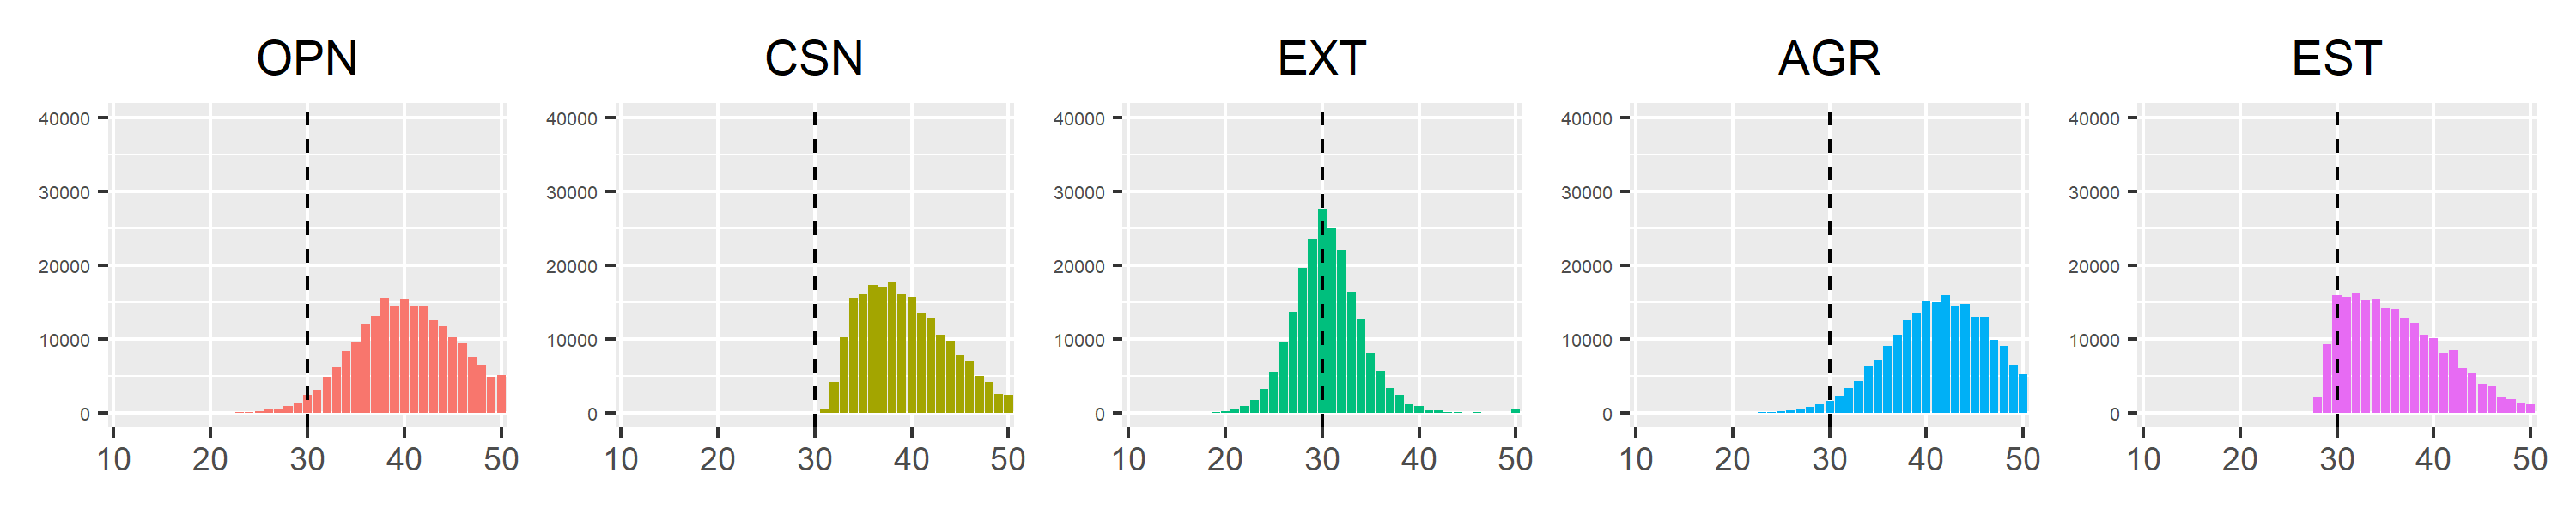
\includegraphics[scale=0.478]{Cluster1.png}
  \caption{类1(206591个样品)的分数分布}
\end{figure}
\begin{figure}[H]
  \centering
  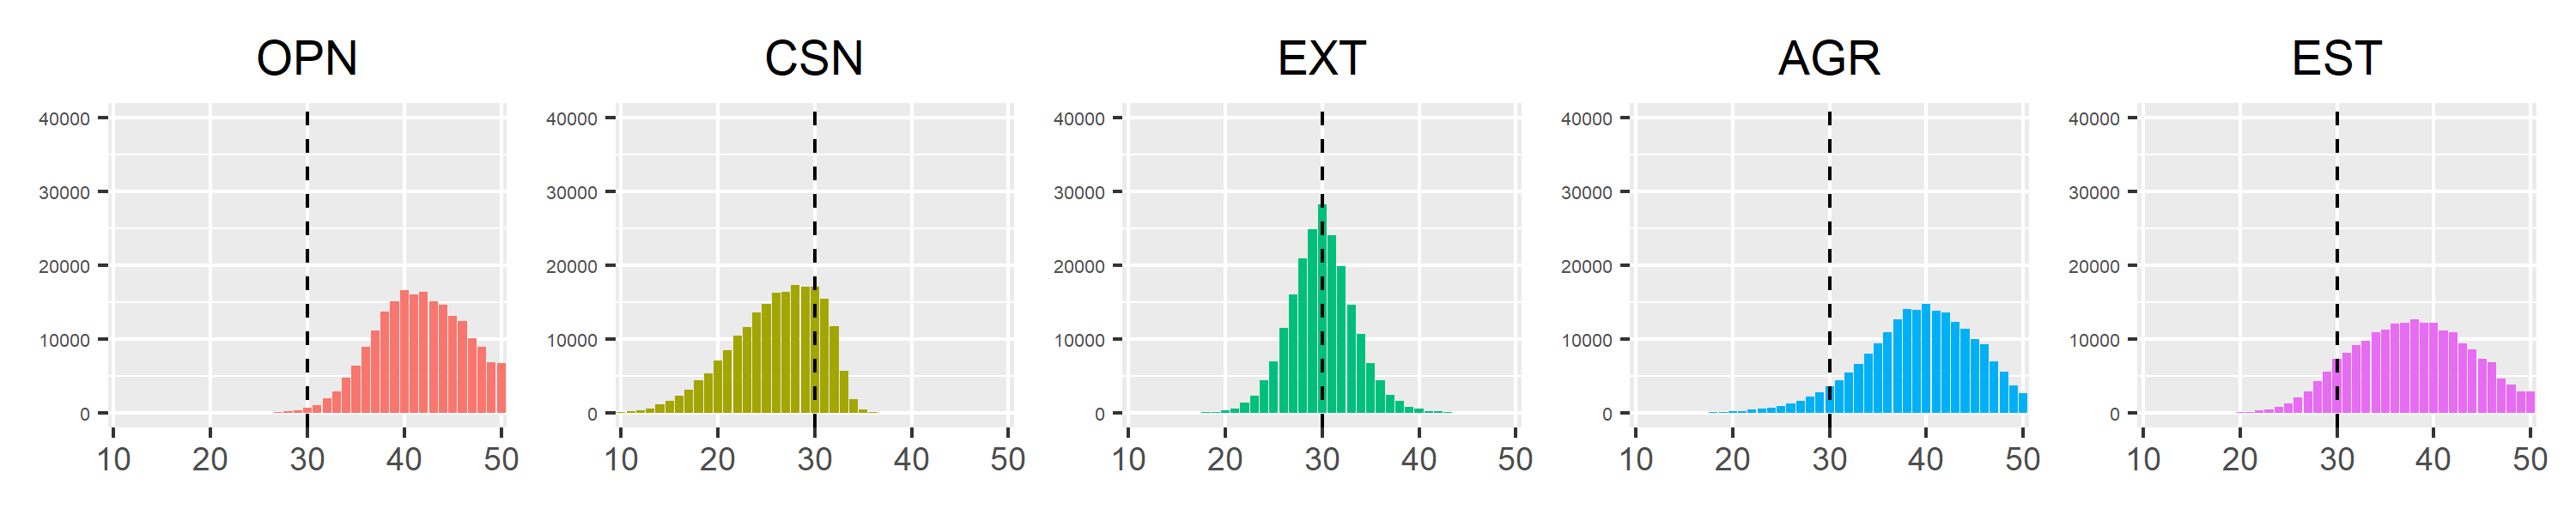
\includegraphics[scale=0.478]{Cluster2.png}
  \caption{类1(204976个样品)的分数分布}
\end{figure}
\begin{figure}[H]
  \centering
  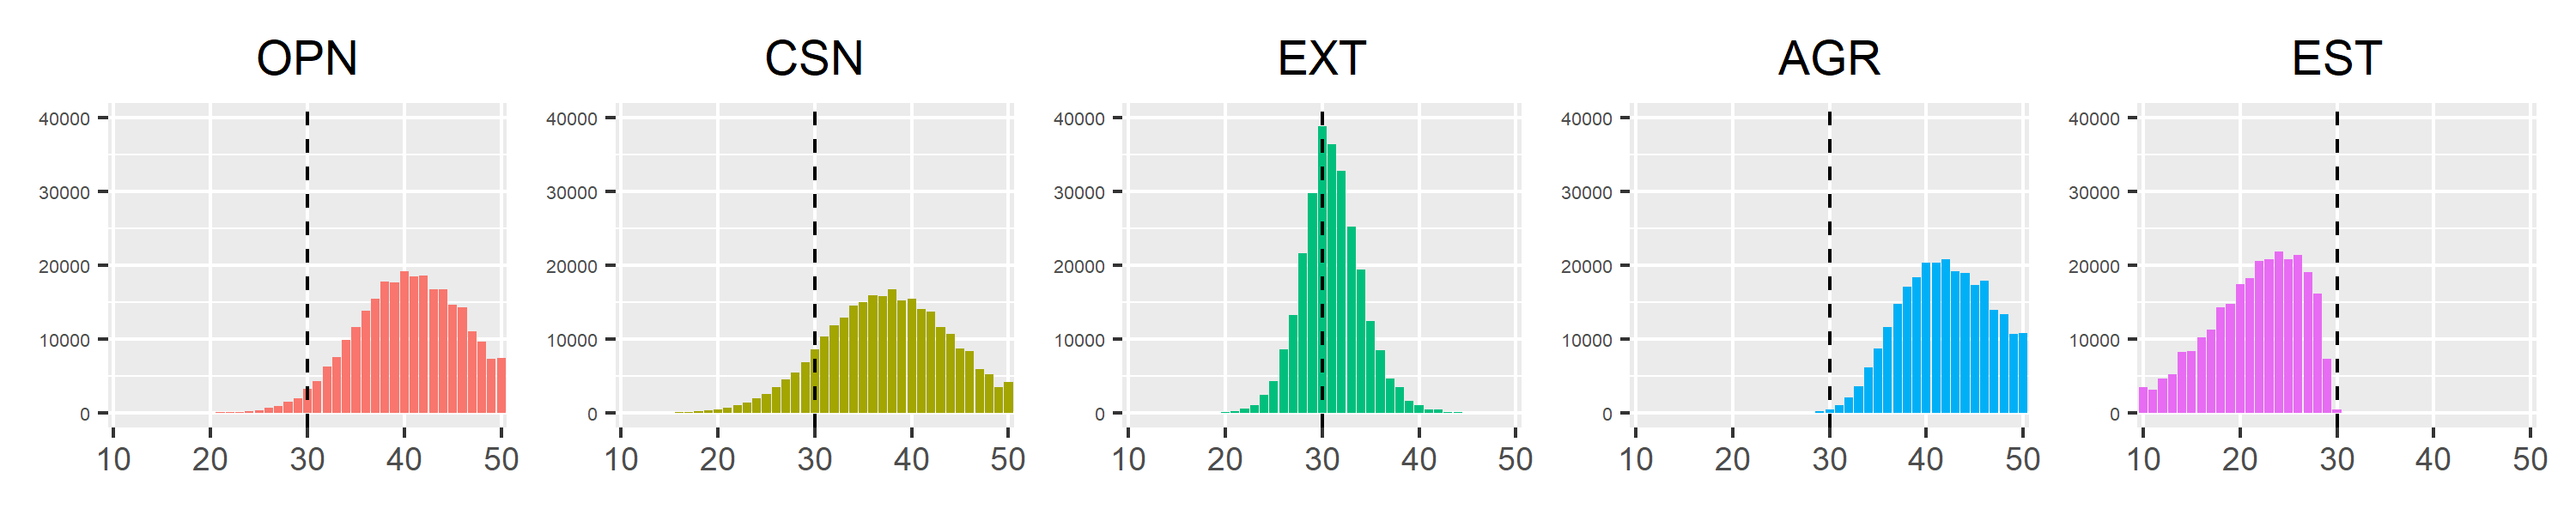
\includegraphics[scale=0.478]{Cluster3.png}
  \caption{类1(268242个样品)的分数分布}
\end{figure}
\begin{figure}[H]
  \centering
  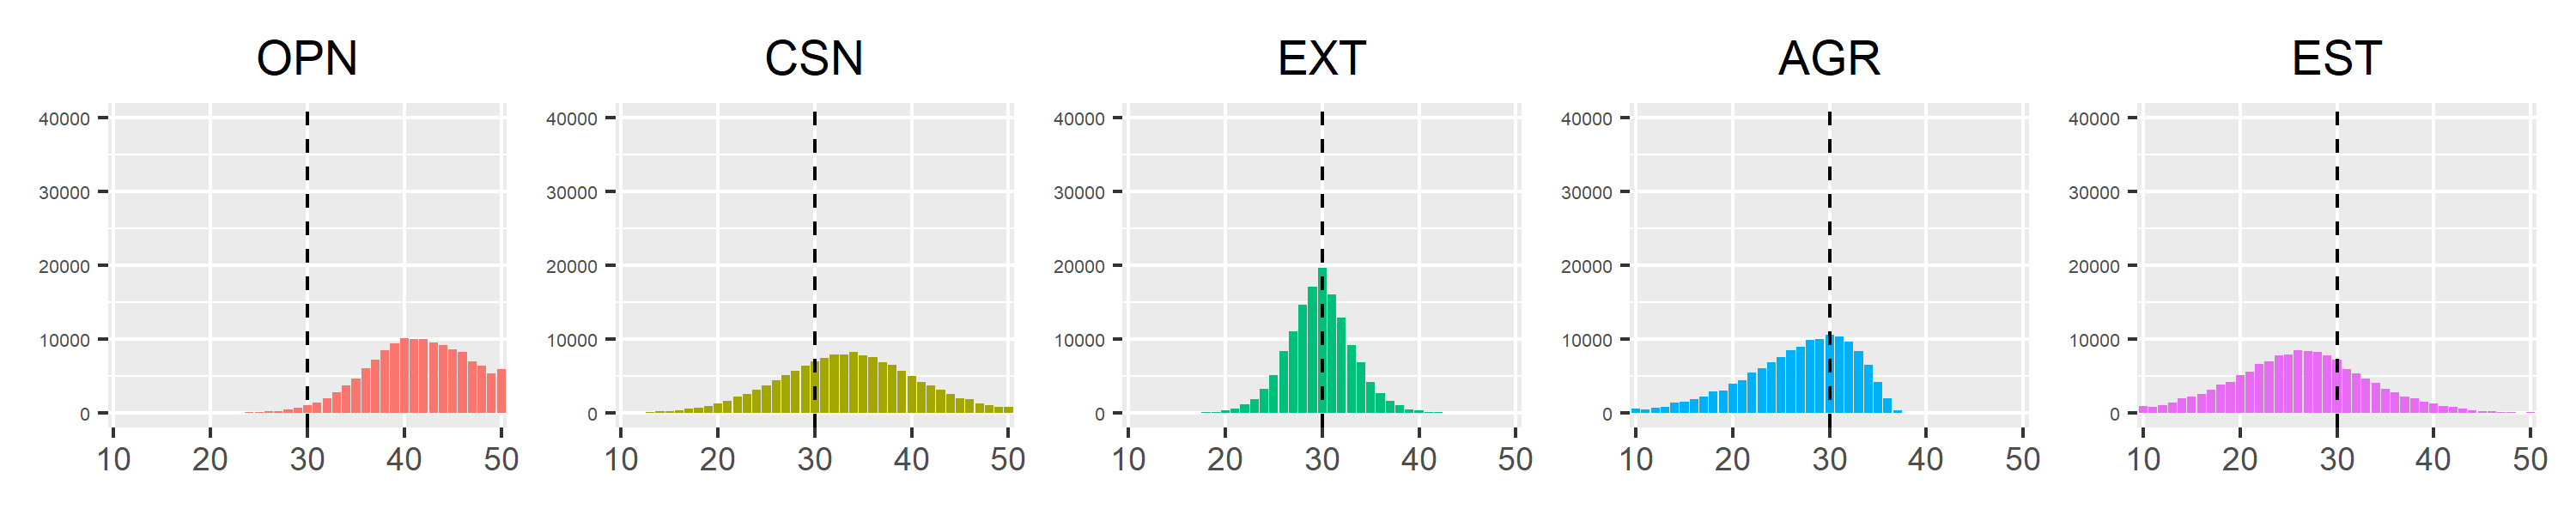
\includegraphics[scale=0.478]{Cluster4.png}
  \caption{类1(139360个样品)的分数分布}
\end{figure}
\begin{figure}[H]
  \centering
  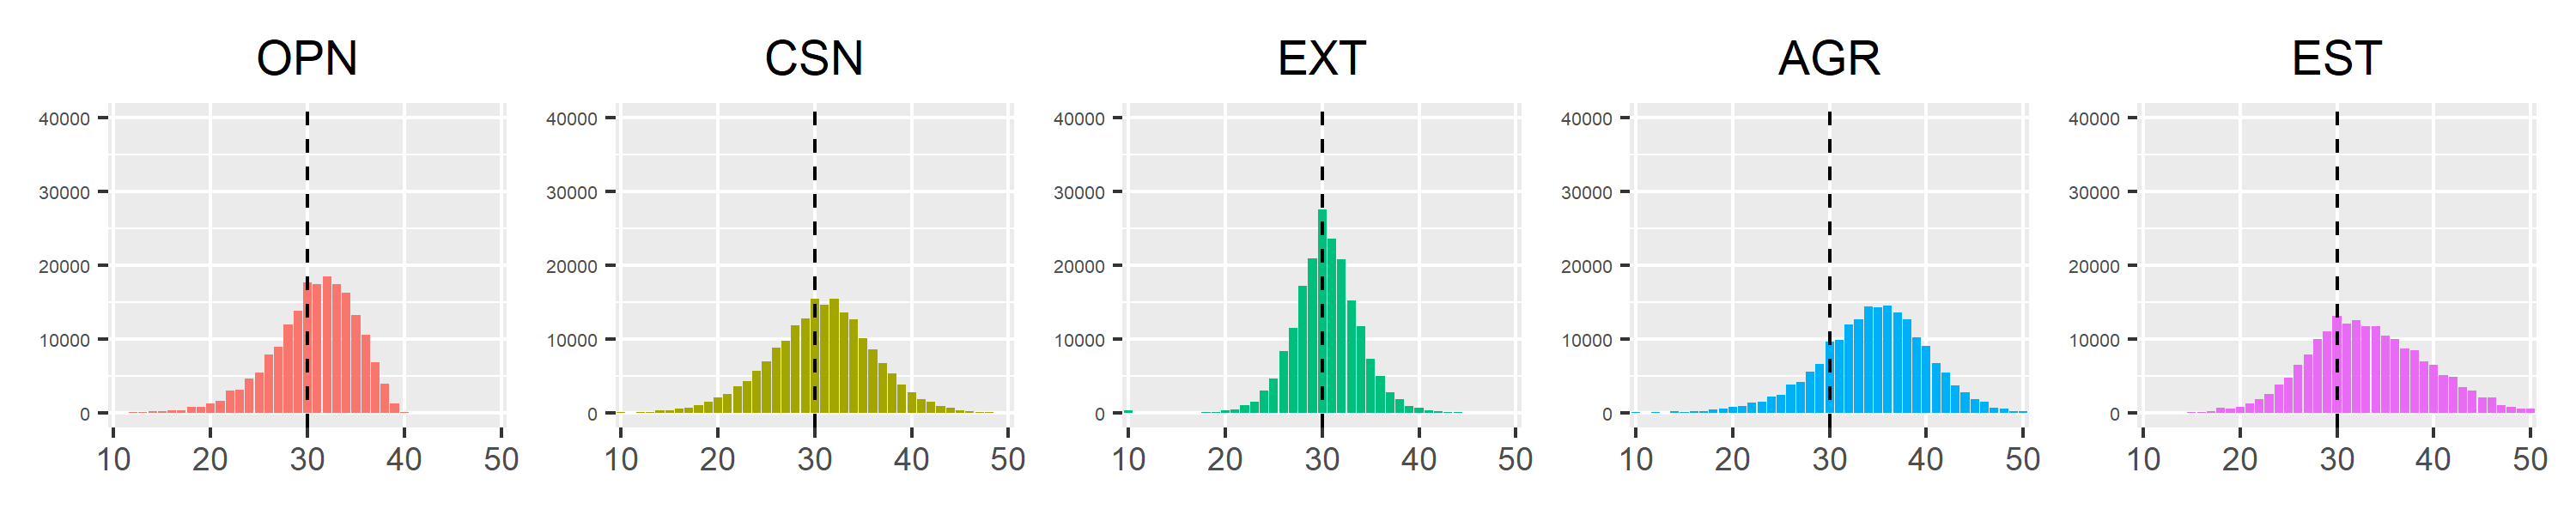
\includegraphics[scale=0.478]{Cluster5.png}
  \caption{类1(189021个样品)的分数分布}
\end{figure}
如图所示,以维度总分的中值30为界,将分布图像分成两个部分,
可以看到在不同的类中,分数的最大密度区间有所不同。
定义“绝大部分”为“80\%”,如果绝大部分样品的维度总分不大于30,记为符号“-”,表示低分倾向;
如果绝大部分样品的维度总分不小于30,记为符号“+”,表示高分倾向;
否则,记为符号“0”,表示中立倾向,可以得到一个关于类的特征的符号矩阵:
\begin{longtable}{c|c|c|c|c|c}
  \hline
  类编号 & OPN & CSN & EXT & AGR & EST \\\hline
  1   & +   & +   & 0   & +   & +   \\
  2   & +   & -   & 0   & +   & +   \\
  3   & +   & +   & 0   & +   & -   \\\hline
  4   & +   & 0   & 0   & 0   & 0   \\
  5   & 0   & 0   & 0   & +   & 0   \\\hline
  \caption{5-均值聚类结果的符号特征}
  \label{symbol5}
\end{longtable}
结合表\ref{center}和表\ref{symbol5},我们能够比较清楚地看出类与类之间的差别和划分依据。
对比类与类之间的维度差异,5个类又可以分为2个大类:
大类1包括类1、类2和类3,主要差异在尽责性维度和宜人性维度,其余维度差别较小;
大类2包括类4和类5,主要差异在开放性维度和宜人性维度,其余维度差别较小。
对比维度在划分类中的重要性,尽责性维度和情绪性维度分出了3种符号,区分了2个大类和大类1中的3个小类;
开放性维度和宜人性维度分出了2种符号,仅区分了大类2中的2个小类。\par
综合前面分数的分布类型来看,尽责性和外倾性是区分不同人格特质的比较重要的维度,
仅以这两个维度上分数的高低表现就可以将参加测验者大致分入4个类中;
开放性和宜人性是在人格特质中区分度较低的维度,绝大部分人在这两个维度上都有高分倾向;
而外倾性维度在5-均值聚类方法中无法有效区分出不同的人格特质类型,
可能需要提高聚类个数进一步提取外倾性维度上的差异。
\section{与十六型人格的对比分析}
不同的人格理论可以看作研究人格的不同角度,那么它们之间是否有一定联系呢?
以目前“类型说”最热门的MBTI十六型人格为例,我们可以将大五人格测验中各维度的分数聚成16个类,
与MBTI的16个人格类型作对比,研究二者之间是否能一一对应或有所联系。\par
使用同样的数据进行16-均值聚类,迭代收敛后,16个类分别为:
\begin{longtable}{c|c|c}
  \hline
  类编号 & 样品数   & 类内平方和    \\\hline
  1   & 57111 & 13566.60 \\\hline
  2   & 63403 & 14298.62 \\\hline
  3   & 73622 & 13247.78 \\\hline
  4   & 36915 & 9864.78  \\\hline
  5   & 42954 & 11207.37 \\\hline
  6   & 64605 & 11102.45 \\\hline
  7   & 71200 & 13757.09 \\\hline
  8   & 61827 & 12023.10 \\\hline
  9   & 71959 & 10064.71 \\\hline
  10  & 47915 & 12236.17 \\\hline
  11  & 41432 & 11026.07 \\\hline
  12  & 83898 & 14471.60 \\\hline
  13  & 67361 & 12172.47 \\\hline
  14  & 83729 & 11454.87 \\\hline
  15  & 71569 & 11765.32 \\\hline
  16  & 68690 & 12915.96 \\\hline
  \caption{16-均值聚类结果}
\end{longtable}
\noindent 其中类的样品数和类内平方和都在同一水平,是一种比较好的划分。每个类的中心为:
\begin{longtable}{c|c|c|c|c|c}
  \hline
  类编号 & OPN   & CSN   & EXT   & AGR   & EST   \\\hline
  1   & 29.34 & 31.02 & 29.88 & 29.65 & 29.23 \\\hline
  2   & 31.34 & 27.86 & 30.57 & 36.29 & 40.91 \\\hline
  3   & 32.27 & 38.31 & 30.81 & 40.15 & 35.45 \\\hline
  4   & 41.99 & 26.02 & 29.78 & 26.39 & 23.46 \\\hline
  5   & 40.61 & 25.05 & 29.01 & 26.94 & 39.99 \\\hline
  6   & 34.52 & 26.22 & 30.98 & 40.01 & 29.33 \\\hline
  7   & 42.93 & 24.27 & 29.83 & 41.56 & 39.93 \\\hline
  8   & 42.55 & 28.91 & 30.78 & 40.60 & 19.81 \\\hline
  9   & 43.26 & 32.21 & 30.80 & 44.83 & 30.07 \\\hline
  10  & 42.08 & 40.17 & 30.18 & 28.21 & 20.69 \\\hline
  11  & 40.82 & 39.53 & 29.27 & 26.57 & 37.30 \\\hline
  12  & 33.76 & 37.97 & 31.03 & 39.79 & 23.25 \\\hline
  13  & 43.00 & 42.37 & 31.20 & 44.20 & 18.03 \\\hline
  14  & 41.51 & 32.96 & 30.50 & 35.17 & 31.73 \\\hline
  15  & 42.12 & 42.98 & 30.70 & 42.94 & 30.07 \\\hline
  16  & 42.47 & 37.13 & 30.12 & 42.14 & 41.60 \\\hline
  % 1   & 40.83 & 39.47 & 29.24 & 26.41 & 37.35 \\\hline
  % 2   & 42.07 & 25.60 & 29.91 & 28.17 & 22.79 \\\hline
  % 3   & 43.21 & 37.76 & 30.06 & 42.26 & 41.10 \\\hline
  % 4   & 41.43 & 25.07 & 29.87 & 41.18 & 41.63 \\\hline
  % 5   & 33.38 & 38.89 & 30.98 & 39.92 & 23.89 \\\hline
  % 6   & 32.61 & 37.70 & 31.04 & 40.14 & 37.04 \\\hline
  % 7   & 41.72 & 25.23 & 29.08 & 27.31 & 38.93 \\\hline
  % 8   & 42.09 & 30.76 & 30.92 & 41.53 & 19.87 \\\hline
  % 9   & 42.27 & 40.11 & 30.15 & 27.90 & 20.70 \\\hline
  % 10  & 33.61 & 27.29 & 31.05 & 40.14 & 29.46 \\\hline
  % 11  & 44.02 & 27.80 & 30.50 & 43.56 & 31.29 \\\hline
  % 12  & 29.77 & 31.52 & 29.88 & 29.44 & 28.33 \\\hline
  % 13  & 42.93 & 42.99 & 31.19 & 44.08 & 17.83 \\\hline
  % 14  & 42.34 & 41.38 & 30.80 & 43.86 & 29.61 \\\hline
  % 15  & 41.05 & 33.89 & 30.59 & 35.48 & 31.41 \\\hline
  % 16  & 30.11 & 27.01 & 30.08 & 34.02 & 40.47 \\\hline
  \caption{16-均值聚类中心}
\end{longtable}
\noindent 同样以30为界,将其转化为符号矩阵:
\begin{longtable}{c|c|c|c|c|c}
  \hline
  类编号 & OPN & CSN & EXT & AGR & EST \\\hline
  1   & 0   & 0   & 0   & 0   & 0   \\
  2   & 0   & 0   & 0   & +   & +   \\
  3   & 0   & +   & 0   & +   & +   \\
  4   & +   & -   & 0   & 0   & -   \\
  5   & +   & -   & 0   & 0   & +   \\
  6   & +   & -   & 0   & +   & 0   \\
  7   & +   & -   & 0   & +   & +   \\
  8   & +   & 0   & 0   & +   & -   \\
  9   & +   & 0   & 0   & +   & 0   \\
  10  & +   & +   & 0   & 0   & -   \\
  11  & +   & +   & 0   & 0   & +   \\
  12  & +   & +   & 0   & +   & -   \\
  13  & +   & +   & 0   & +   & -   \\
  14  & +   & +   & 0   & +   & 0   \\
  15  & +   & +   & 0   & +   & 0   \\
  16  & +   & +   & 0   & +   & +   \\\hline
  \caption{16-均值聚类结果的符号特征}
  \label{symbol16}
\end{longtable}
从表\ref{symbol16}中能够发现16个类对于大五人格测验的数据来说有些多了,
类12和类13、类14和类15没有足够明显的特征差异,从大五人格测验的数据中划分出16个类型还是有困难的,
但我们可以从16-均值聚类的结果中得到一些有用的信息。\par
首先,在提高到16个类后,外倾性维度在各个类之间的区分度依旧很低。
一种可能的情况是,一个人对外的性格表现为热情或是冷静,与其他四个维度的倾向性没有关联,
外倾性是作为一个独立的指标,给出测试者对外界积极性的度量。\par
其次,开放性维度和宜人性维度也没有分离出典型低分倾向的类。
通过维度和题目的描述我们能看出来,在开放性维度和宜人性维度上有高分倾向的人,
正是社会中比较受欢迎的类型——思想活跃、容易相处,也有很多人想把自己改造为这样的类型;
而老实本分的人多少有些沉闷,斗争性强的人则普遍评价不会太高,社会留给他们的位置相对更少一些。
这种环境下,两个维度出现大量高分倾向的人也就不足为奇了。\par
最后,区分度最好的维度还是尽责性维度和情绪性维度。
如果将社会比作一部机器,尽责性维度上的高分人群构成了机器的骨架,低分人群则是润滑剂,
二者都在维系机器正常运行中发挥着作用。
“情绪化”一词更像是一个中性词,它如何发挥作用取决于外部条件。
艺术创作需要丰富的情绪来激发灵感,体育运动需要刺激兴奋来激发潜力,
学习研究需要适当的压力来推动进度,而任何时候面对突发情况都需要一颗清醒的头脑去处理问题。
因此,社会对在尽责性维度和情绪性维度上具有高分或低分倾向的人有着更高的容忍度,
可以比较容易地划分出他们所属的类群。\par
对于MBTI十六型人格,其优势是测验结果可以简单地用4个字母概括,极大地方便了传播,
但是缺点也很明显
\end{document}